\def\showSarcasticRemarks{}
\def\showTODOs{}

\documentclass[a4paper,UKenglish,cleveref, autoref]{lipics-v2019}
\usepackage{proof}
\usepackage{tikz}
\usepackage{gensymb}
\usepackage{enumitem}
\usepackage{booktabs}


\usetikzlibrary{automata,trees,calc,arrows.meta,positioning,decorations.pathreplacing,bending,shapes.geometric, intersections, hobby}



%This is a template for producing LIPIcs articles. 
%See lipics-manual.pdf for further information.
%for A4 paper format use option "a4paper", for US-letter use option "letterpaper"
%for british hyphenation rules use option "UKenglish", for american hyphenation rules use option "USenglish"
%for section-numbered lemmas etc., use "numberwithinsect"
%for enabling cleveref support, use "cleveref"
%for enabling cleveref support, use "autoref"

%\graphicspath{{./graphics/}}%helpful if your graphic files are in another directory

\bibliographystyle{plainurl}% the mandatory bibstyle

\title{Towards a Formalisation of Cook's Theorem} %TODO Please add

\titlerunning{}%optional, please use if title is longer than one line

\author{Lennard Gäher}{Saarland University, Germany}{s8legaeh@stud.uni-saarland.de}{}{}%TODO mandatory, please use full name; only 1 author per \author macro; first two parameters are mandatory, other parameters can be empty. Please provide at least the name of the affiliation and the country. The full address is optional

\authorrunning{L. Gäher}%TODO mandatory. First: Use abbreviated first/middle names. Second (only in severe cases): Use first author plus 'et al.'

\Copyright{Lennard Gäher}%TODO mandatory, please use full first names. LIPIcs license is "CC-BY";  http://creativecommons.org/licenses/by/3.0/

%\ccsdesc[100]{General and reference~General literature}
%\ccsdesc[100]{General and reference}%TODO mandatory: Please choose ACM 2012 classifications from https://dl.acm.org/ccs/ccs_flat.cfm 

%\keywords{Dummy keyword}%TODO mandatory; please add comma-separated list of keywords

%\category{}%optional, e.g. invited paper

\relatedversion{}%optional, e.g. full version hosted on arXiv, HAL, or other respository/website
%\relatedversion{A full version of the paper is available at \url{...}.}

\supplement{}%optional, e.g. related research data, source code, ... hosted on a repository like zenodo, figshare, GitHub, ...

%\funding{(Optional) general funding statement \dots}%optional, to capture a funding statement, which applies to all authors. Please enter author specific funding statements as fifth argument of the \author macro.


\nolinenumbers %uncomment to disable line numbering

\hideLIPIcs  %uncomment to remove references to LIPIcs series (logo, DOI, ...), e.g. when preparing a pre-final version to be uploaded to arXiv or another public repository

%Editor-only macros:: begin (do not touch as author)%%%%%%%%%%%%%%%%%%%%%%%%%%%%%%%%%%
\EventEditors{John Q. Open and Joan R. Access}
\EventNoEds{2}
\EventLongTitle{42nd Conference on Very Important Topics (CVIT 2016)}
\EventShortTitle{CVIT 2016}
\EventAcronym{CVIT}
\EventYear{2016}
\EventDate{December 24--27, 2016}
\EventLocation{Little Whinging, United Kingdom}
\EventLogo{}
\SeriesVolume{42}
\ArticleNo{23}
%%%%%%%%%%%%%%%%%%%%%%%%%%%%%%%%%%%%%%%%%%%%%%%%%%%%%%

\usepackage{gensymb}
\newcommand*{\listsofb}[1]{\mathcal{L} (#1)}
\newcommand*{\listsof}{\mathcal{L}~}

\newcommand{\None}{\emptyset}
\newcommand{\Some}[1]{\degree\kern-0.5ex#1}

\newcommand*{\match}{\textbf{match}~}
\newcommand*{\withl}{\textbf{[}~}
\newcommand*{\withr}{~\textbf{]}}
\newcommand*{\withm}{\quad\textbf{|}\quad}
\newcommand*{\llet}{\textbf{let}~}
\newcommand*{\lin}{\textbf{in}~}
\newcommand{\ITE}[3]{\textbf{if}~{#1}~\textbf{then}~{#2}~\textbf{else}~{#3}}

\newcommand{\Type}{\textsf{\bfseries T}}
\newcommand{\Prop}{\textsf{\bfseries P}}
\newcommand{\bool}{\textsf{B}}
\newcommand{\btrue}{\mathsf{T}}
\newcommand{\bfalse}{\mathsf{F}}
\newcommand{\andb}{\&\&}
\newcommand{\orb}{||}
\newcommand{\notb}{!}
\newcommand{\nat}{\mathsf{N}}
\newcommand{\natS}{1 + }
\newcommand{\length}[1]{|#1|}

\newcommand{\con}{\mathop{{+}\!\!\!{+}}}
\newcommand{\rev}{\mathsf{rev}}
\newcommand{\opt}[1]{\mathcal{O}{#1}}
\newcommand{\nil}{[]}

\newcommand{\eqb}[2]{#1\overset{?}{=}#2}

\newcommand{\bnfmid}{~\mid~}

\newcommand{\concat}{\con}


\newcommand{\TODO}[1]{\ifthenelse{\isundefined{\showTODOs}}{}{\colorbox{red}{\LARGE TODO}:#1}}
\newcommand{\sarcasm}[1]{\ifthenelse{\isundefined{\showSarcasticRemarks}}{}{\footnote{#1}}}

\newcommand{\strent}{\rightsquigarrow}
\newcommand{\constrent}{\overset{!}{\rightsquigarrow}}
\newcommand{\Rfinal}{R_{\text{final}}}

\newcommand{\bigO}[1]{\mathcal{O}{(#1)}}

\begin{document}

\maketitle

%TODO mandatory: add short abstract of the document
\begin{abstract}
  We present an outline of the planned proof of Cook's Theorem in Coq.
\end{abstract}

\newcommand{\gennp}{\textbf{GenNP}}
\newcommand{\strconrew}{\textbf{PR}}
\newcommand{\binstrconrew}{\textbf{BinPR}}
\newcommand{\csat}{\textbf{FSAT}}
\newcommand{\sat}{\textbf{SAT}}
\newcommand{\NP}{\textsf{NP}}

\newcolumntype{C}{>{$}c<{$}}
\newcommand{\rewwin}[2]{
  \begin{tabular}{C|C|C}
    #1 \\ 
    \midrule #2
  \end{tabular}
}

\newcommand{\blank}{\textbf{\textvisiblespace}}

\section{Introduction}
Cook's Theorem was proved in 1971 by Stephen A.\ Cook (and, in parallel, by Levin) and is one of the foundational results of computational complexity theory. 
It states that the satisfiability problem on CNFs \textbf{SAT} is NP-hard, that is, any problem $Q \in NP$ can be polynomial-time reduced to it: $Q \prec_{\text{p}} \textbf{SAT}$. 
There are multiple well-known textbook proofs available. We strive to adapt a particularly simple one which encodes the transitions of a Turing machine using logical formulas layed out in a tableau.
An outline of this classical proof can be found in~\cite{Sipser:TheoryofComputation}. 

Despite the conceptual simplicity of the original proof, the formalisation is quite demanding. The key difficulties lie with 
\begin{itemize}
  \item encoding nondeterminism, 
  \item working with our particular representation of Turing machine tapes,
  \item reserving enough space for the Turing machine beforehand since the logical formula must have a fixed size,
  \item ensuring time bounds.
\end{itemize}

Our reduction has the following structure: 
\begin{center}
  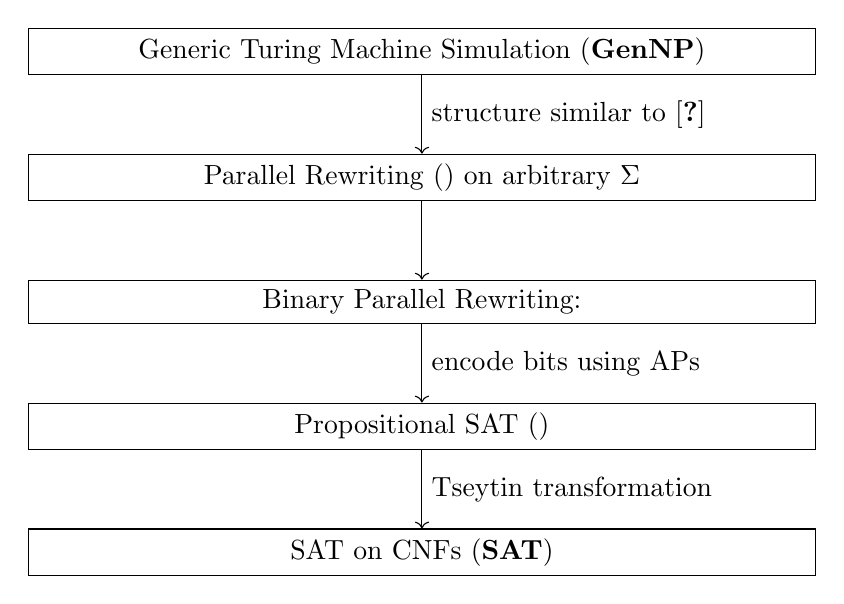
\begin{tikzpicture}
    \node[rectangle, draw=black, minimum width = 10cm] (gennp) {Generic Turing Machine Simulation (\textbf{GenNP})};
    \node[rectangle, draw=black, below = of gennp, minimum width = 10cm] (strrew1) {Parallel Rewriting (\strconrew) on arbitrary $\Sigma$};
    \node[rectangle, draw=black, below = of strrew1, minimum width = 10cm] (strrew2) {Binary Parallel Rewriting: \binstrconrew};
    \node[rectangle, draw=black, below = of strrew2, minimum width = 10cm] (csat) {Propositional SAT (\csat{})};
    \node[rectangle, draw=black, below = of csat, minimum width = 10cm] (sat) {SAT on CNFs (\textbf{SAT})};
    \draw[->] 
      (gennp) edge node[right] {structure similar to~\cite{Sipser:TheoryofComputation}} (strrew1)
      (strrew1) edge (strrew2)
      (strrew2) edge node[right] {encode bits using APs} (csat)
      (csat) edge node[right] {Tseytin transformation} (sat);
  \end{tikzpicture}
\end{center}

The reduction from \gennp{} to \strconrew{} does the main job of encoding the behaviour of Turing machines. We are then left with a structurally much simpler problem on strings. 
In order to be able to encode this problem using logical formulas, we then simplify the alphabet to $\{0, 1\}$ in a reduction to \binstrconrew, making it possible to encode single characters using a boolean-valued atomic proposition in the reduction to \csat. The encoding of the string rewriting system that we use will not be in conjunctive normal form (CNF), therefore we then use the Tseytin transformation in a reduction from \csat{} to \sat{} on CNFs. 

%\TODO{consider introducing two new problems before strconrew that are already working with rewriting systems, but factor out the need to ``guess'' initial strings (first part: reduction to ``exists tape'', second part: reduction to ``exists tape whose position is normalised'', then reduction to strconrew)}

\section{Involved Languages}
We first give a formal description of the involved problems. 

\subsection{Generic Turing Machine Simulation (\gennp{})}\label{sec:TM}
The formalisation of Turing machines we use has been introduced in~\cite{ForsterEtAl:2019:VerifiedTMs}, although we do not have any use for the abstractions developed for the programming of Turing machines in Coq. This formalisation is based on one originally done in the proof assistant Matita~\cite{Asperti2015AFO}. 

For the representation of tapes, no blank symbol is explicitly specified. Instead, the constructors explicitly specify whether the head is currently at the left or the right end of the used tape area.
\begin{definition}[Tapes] \label{def:tapes}
  Let $\Sigma$ be a type. A tape is defined by
  \[\textsf{Tape}_\Sigma ::= \textsf{niltape} \bnfmid \textsf{leftof}~r~rs \bnfmid \textsf{midtape}~ls~m~rs \bnfmid \textsf{rightof}~l~ls \]
  with $l, m, r : \Sigma$ and $rs, ls : \listsof{\Sigma}$. 
\end{definition}

For each possible tape state and head position, this admits a unique representation: $\textsf{niltape}$ specifies that the tape is completely empty, $\textsf{midtape}~ls~m~rs$ is used when the head currently resides on the symbol $m$ and there are possibly further symbols to the left ($ls$) or right ($rs$). $\textsf{leftof}$ and $\textsf{rightof}$ indicate that the head is currently one symbol to the left or right of the already used tape $l::ls$ or $r::rs$, respectively. 
$ls$ and $rs$ are ordered such that the symbol closest to the head is at the head of the list. 

\begin{definition}[Turing machines]
  An $n$-tape Turing machine $M : \textsf{TM}_\Sigma^n$ over a finite alphabet $\Sigma$ is a tuple $M = (Q, \delta, \mathit{start}, \mathit{halt})$, where $Q$ is the finite type of states, $\delta : Q \times {(\opt{(\Sigma)})}^n \rightarrow Q \times {(\textsf{Act}_\Sigma)}^n$ (with actions $\textsf{Act}_\Sigma := \opt{(\Sigma)} \times \textsf{Move}$ and $\textsf{Move} ::= L \bnfmid R \bnfmid N$) is the transition function, $\mathit{start} : Q$ is the initial state and $\mathit{halt} : Q \rightarrow \bool$ represents the halting states. 
\end{definition}

We now give the basics of the semantics of Turing machines. Let us fix an alphabet $\Sigma$ and a $n$-tape Turing machine $M$.
A single action of the Turing machine on a tape is executed by the function $\textsf{doAct} : \textsf{Tape}_\Sigma \rightarrow \textsf{Act} \rightarrow \textsf{Tape}_\Sigma$, the definition of which can be found in the appendix. This can be extended canonically to a function $\textsf{doAct}$ acting on a vector of tapes.

Configurations of the Turing machine $M$ are defined as pairs of a state and a vector of tapes: $\textsf{Conf}_M : Q \times {(\textsf{Tape}_\Sigma)}^n$. One computational step of $M$ is then executed by the function $\textsf{step}_M : \textsf{Conf}_M \rightarrow \textsf{Conf}_M$. We will denote the induced relation on configurations by $c_1 \succ c_2$.

The function $\textsf{loop}_M : \textsf{Conf}_M \rightarrow \nat \rightarrow \opt{(\textsf{Conf}_M)}$ can then be used to simulate $M$ for a given number of steps. If the Turing machine halts, starting from $c_1$, in a halting configuration $c_2$ within this number of steps, written $c_1 \rhd c_2$, it returns $c_2$, otherwise it returns $\None$.


\begin{definition}[\gennp{}]
  Given a deterministic 1-tape Turing machine $M$ and numbers $k$ and $t$, decide whether there is an input $x$ of length $\length{x} \le k$ such that $M$ halts on $x$ in at most $t$ steps: 
  $\exists c, (\mathit{start}, \textsf{initTape}~x) \rhd^{\le t} c$
  where 
  \begin{align*}
    \textsf{initTape}~\nil := \textsf{niltape}\\
    \textsf{initTape}~(x :: xs) := \textsf{leftof}~x~xs
  \end{align*}
\end{definition}

A more wide-spread (but equivalent) definition of a generic problem for Turing machines is the following: Given a nondeterministic Turing machine $M$ and an input $x$ and a number $t$, decide whether $M$ halts on $x$ in at most $t$ steps. 
We do not use this variant since it would require us to formalise the notion of nondeterminism. Instead, our definition builds on the well-known verifier characterisation of \NP{}. The whole input of the Turing machine is regarded as a certificate; the instance itself can be statically encoded in the states of the Turing machine.

The restriction to 1-tape Turing machines is without loss of generality, a fact which has also been formalised in Coq~\cite{ForsterEtAl:2019:VerifiedTMs}. 

Using a classical definition of the complexity class \NP{} using Turing machines, one is easily convinced that \gennp{} is \NP{}-hard. For our definition using the call-by-value $\lambda$-calculus L, this isn't straightforward at all, though. We thus leave the problem of proving the \NP{}-hardness of \gennp{} open for now.

\subsection{Parallel Rewriting (\strconrew{})}
This problem works on strings of a fixed length $l$ over an alphabet $\Sigma$. Starting with an initial string $x_0$, the task is to determine whether there is a sequence of strings $x_1, \ldots, x_t$ such that $x_{i+1}$ validly follows from $x_i$, denoted by $x_i \strent x_{i+1}$, such that $x_t$ satisfies a final condition. The number $t$ is fixed. All of the strings in the sequence must have the same length $l$. The relation $x_i \strent x_{i+1}$ is described by a set $R$ of rewrite windows.

Each window specifies a rewrite $a \constrent b$ for strings $a, b$ of a fixed length $w \le l$. In order for $x_i \strent x_{i+1}$ to hold, each of the characters of $x_{i+1}$ must be derived from $x_i$ using a rewrite window.
More precisely, in order for a string $x_{i+1}$ to validly follow from a string $x_i$, for each offset $j \cdot o$ in $x_i$ which is a multiple of a rewriting offset $o$, a rewrite window must hold:
\[\bigwedge_{0 \le j\cdot o \le l - w + 1} \bigvee_{(a \constrent b) \in R} (x_i[j\cdot o..j\cdot o+w-1] = a \land x_{i+1}[j\cdot o..j\cdot o+w-1] = b) \]

The final condition is given by a set of substring constraints $\Rfinal$: In order for the final string $x_t$ to be valid, there needs to be $x \in \Rfinal$ such that $x$ is a substring of $x_t$:
\[\bigvee_{x \in \Rfinal} \bigvee_{0 \le j \le l - \length{x} + 1} (x_t[j..j+\length{x} -1] = x) \]

\newcommand*{\validR}{\textsf{valid}}

%\begin{example}[Generating permutations]
  %In this example, we develop an instance of \strconrew{} that determines whether $aaabc$ is a permutation of $abaca$ which can be obtained with at most 10 transpositions. 

  %We work over the alphabet $\Sigma = \{a, b, c\}$ and a string length of $5$. We start with the initial string $x_0=abaca$ and our final substring constraint is $\{aaabc\}$; that is, we require that $aaabc$ is a substring of the final string, which implies equality because the final string will have a length of $5$.

  %Our rewrite windows have a width of 3 characters and we use an offset $o =1$. They allow for exchanging two adjacent characters and thus each rewrite step will capture . Namely, we have the following rewrite windows where $\sigma$ ranges over $\Sigma$:
  %\TODO{more suitable example where the limit in the number of steps has a meaning}
%\end{example}
    
We now formally define \strconrew{}:
\begin{definition}\label{def:strconrew}
  Given: 
  \begin{itemize}
    \item an alphabet $\Sigma$
    \item a string length $l$,
    \item a step count $t$,
    \item an initial string $x_0 \in \Sigma^l$,
    \item a width $w$ of rewrite windows, 
    \item a rewriting offset $o$
    \item a list of rewrite windows $R = \{a_i \constrent b_i | i \in \nat \land a_i, b_i \in \Sigma^w\}$,
    \item a set of final substring constraints $\Rfinal = \{f_i | i \in \nat \land \exists k \le l, f_i \in \Sigma^k\}$
  \end{itemize}

  Determine if there is a sequence of strings $x_1, \ldots, x_t \in \Sigma^l$ such that 
  \begin{itemize}
    \item For every $0 \le i < t$ it holds that $\validR(x_i, x_{i+1})$, where $\validR$ is defined as follows:
      \[\forall (0 \le j\cdot o \le l -w + 1), \exists (a \constrent b) \in R, x_i[j\cdot o..j\cdot o+ k-1] = a \land x_{i+1}[j\cdot o..j\cdot o+k-1] = b \]
      We will denote $\validR(x_i, x_{i+1})$ by $x_i \strent{} x_{i+1}$. 
    \item There exists an $x \in \Rfinal$ such that $x$ is a substring of $x_t$, i.e.\ there is $0 \le j \le l - \length{x} + 1$ with $x = x_t[j..j+\length{x} - 1]$.
      In this case, we may write $x_t \models \Rfinal$.
  \end{itemize}

  A rewriting system is specified by an 8-tuple $S = (\Sigma, l, t, x_0, w, o, R, \Rfinal)$.
\end{definition}

We admit that this definition is quite complex, but hope that the reason for this complexity becomes clear in the reduction from \gennp{}.
Usually, we will use triples $S = (x_0, R, \Rfinal)$ to refer to a rewriting system; all the other parameters will be clear from the context.

Moreover, we will also use the notation $x \strent{} y$ for strings $x, y$ with $\length{x} = \length{y} < l$ in the natural way, by requiring that only for all positions $j$ with $0 \le j \cdot o \le \length{x} - w + 1$ a rewrite window holds. This allows us to reason about rewrites in substrings of a rewriting system. 
In some contexts, we will restrict the relation $\strent{}$ to only use rules from a set $R'$. We will denote this restriction by $\strent{}_{R'}$.

A rewriting system is deterministic for a class of strings if there is at most one successor for these strings according to the relation $\strent{}$:
\begin{definition}[Determinism]\label{def:rewdet}
  Let a rewriting system $S = (\Sigma, l, t, x_0, w, o, R, \Rfinal)$ and a predicate $p : \listsofb{\Sigma} \rightarrow \Prop$ be given. 
  $S$ is deterministic for $p$, iff: 
  \[ \forall s, p~s \rightarrow \forall s_1~s_2, s \strent{} s_1 \rightarrow s \strent{} s_2 \rightarrow s_1 = s_2 \]
\end{definition}

%This is equivalent to the derivation being unique:
%\begin{lemma}
  %A rewriting system $S$ is deterministic for $p$, iff $\mathcal{W}($
%\end{lemma}

Finally, we establish a few properties about \strconrew{}. For the remainder of this section, fix a rewriting system with parameters according to Definition~\ref{def:strconrew}.

\begin{lemma}\label{lem:rewind}
  $a :: b :: c :: rs \strent{} a' :: b' :: c' :: rs'$ iff $b :: c :: rs \strent{} b' :: c' :: rs'$ and $abc \constrent{} a'b'c'$. 
\end{lemma}
This lemma enables us to prove rewrites inductively. Note that we are already using the notational convention for $\strent{}$ established above.

\subsection{Binary Parallel Rewriting (\binstrconrew{})}
\TODO{}

\subsection{Propositional Satisfiability (\csat{})}
\newcommand{\var}{\textsf{var}}
\newcommand{\literal}{\textsf{literal}}
\newcommand{\clause}{\textsf{clause}}
\newcommand{\cnf}{\textsf{cnf}}
\newcommand{\assgn}{\textsf{assgn}}
\newcommand{\eval}[2]{\mathcal{E}~#1~#2}
\newcommand{\for}{\textsf{For}}


In the \csat{} problem, we consider formulas over atomic propositions $x : \var := \nat$. Starting from atomic propositions, larger formulas can be built using negation $\lnot$ and binary as well as $n$-ary conjunction $\land$ and disjunction $\lor$. The choice to incorporate binary and $n$-ary versions of the operators is merely for convenience, we could restrict ourselves to either of them, although $n$-ary versions will be quite convenient in the reduction of \csat{} to \sat{} (Section~\ref{TODO}). 

More formally, we define: 
\begin{align*}
  f : \for := x \bnfmid f_1 \lor f_2 \bnfmid f_1 \land f_2 \bnfmid f_1 \lor f_2 \lor \ldots \lor f_n \bnfmid f_1 \land f_2 \land \ldots \land f_n \bnfmid \lnot f \quad (x : \var)
\end{align*}

Boolean values can be assigned to atomic propositions; the formula can then be evaluated under such an assignment in the canonical way using Boolean operators. 
We model assignments as lists of Boolean values:
\[ a : \textsf{assgn} := \listsofb{\bool}\]
The value at position $i$ of a list $a$ corresponds to the value assigned to atomic proposition $i$. Thus, if an assignment is too short, it may fail to assign a value to some of the atomic propositions of a formula $f$. Evaluation is thus partial.
We believe that the added expressivity of this approach versus a definition of assignments using default values for unassigned atomic propositions is worth the drawback of partiality.

We define an evaluation function $\mathcal{E} : \assgn \rightarrow \for \rightarrow \opt{(\bool)}$ in the canonical way. The option type encodes the partiality observed above. 

Now the problem \csat{} asks, given a formula $f$, if there exists an assignment $a$ that satisfies $f$, that is, $\eval{a}{f} = \Some{\btrue}$. 
\begin{definition}[Propositional Satisfiability \csat{}]
  \[\csat{}~f := \exists~a, \eval{a}{f} = \Some{\btrue}  \]
\end{definition}

\subsection{Satisfiability of CNFs (\sat{})}

The satisfiability problem on CNFs is a special case of the general \csat{} formulation. Here, the formula needs to be in conjunctive normal form: 
\begin{align*}
  x : \var := \nat &&
  L : \literal := \bool \times \var &&
  C : \clause := \listsof \literal &&
  N : \cnf := \listsof \clause && 
\end{align*}

At the innermost level, we have literals which are either atomic propositions or negations of atomic propositions. Clauses are disjunctions of literals and finally, a CNF is a conjunction of clauses.

We will use the same notion of assignments as for formulas $\for$. 
Evaluation functions $\mathcal{E}$ can be defined for literals, clauses and CNFs in a similar way as for $\for$. We will refer to all of these functions with the same letter $\mathcal{E}$, but from the context it will always be clear what we mean.

A more formal treatment of our definition of CNFs can be found in~\ref{memo1}.

The problem \sat{} asks if a given CNF is satisfiable:
\begin{definition}
  \[\sat{}~N := \exists~a, \eval{a}{N} = \Some{\btrue} \]
\end{definition}


\section{Reducing \gennp{} to \strconrew{}}
The basic idea of this reduction is very similar to the reduction in~\cite{Sipser:TheoryofComputation}, although we encode Turing machines using a constrained string rewriting system instead of logical formulas. We defer the handling of nondeterministically ``guessing'' an input of size at most $k$ to Section~\ref{sec:nondet} and instead first deal with a setting in which we are given a deterministic 1-tape Turing machine and a fixed input $\sigma_1, \ldots, \sigma_k$ of size $k$. 

Let us fix a Turing machine $M$ over $\Sigma$ throughout this section. 

\subsection{Encoding Deterministic Turing Machines}
The configurations of the Turing machine are laid out in a tableau of $t \cdot (1 + 2(k + t + 3))$ characters. Each configuration is modelled by one line of the tableau, that is, a string of length $1 + 2(k + t + 3)$. Starting from an initial configuration $x_0$, the transition function is then encoded using rewrite windows of width 3 and rewriting offset 1. The final constraint is that the final configuration contains the symbol of a halting state. 
Using the string rewriting problem, it is then determined whether there exists an execution of the Turing machine for which it halts after at most $t$ steps. 

\begin{center}
  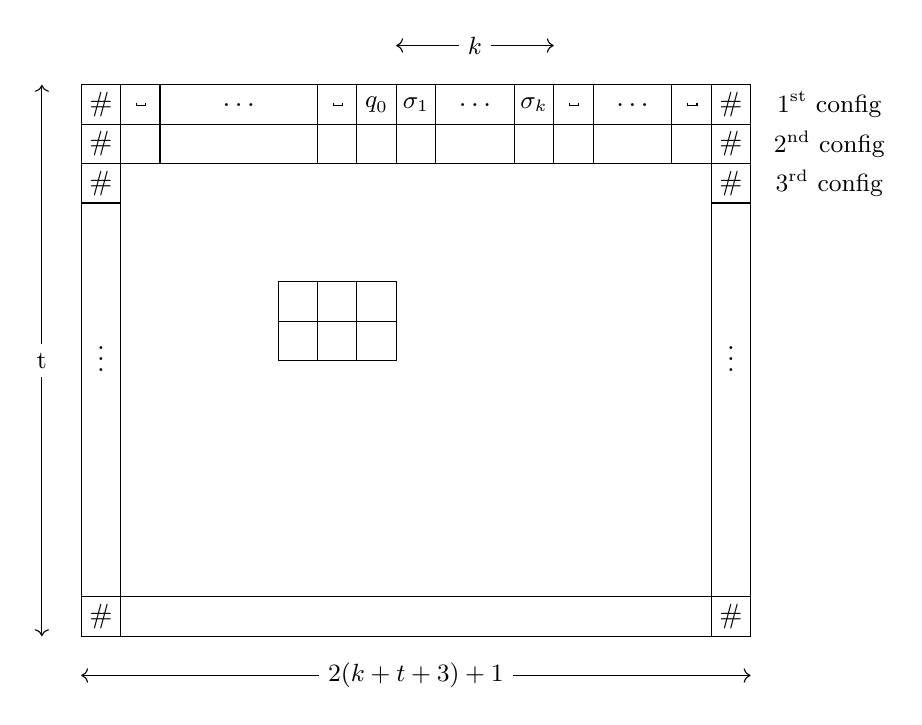
\begin{tikzpicture}
    \draw (1.5, -4) -- (1.5, 3) -- (10, 3) -- (10, -4) -- (1.5, -4);
    \draw (2, -4) -- (2, 3);
    \draw (2.5, 3) -- (2.5, 2);
    \draw (9.5, -4) -- (9.5, 3);
    \draw (1.5, 2.5) -- (10, 2.5);
    \draw (1.5, -3.5) -- (10, -3.5);
    \draw (1.5, 2) -- (10, 2);
    \draw (1.5, 1.5) -- (2, 1.5);
    \draw (9.5, 1.5) -- (10, 1.5);

    \draw (4.5, 3) -- (4.5, 2);
    \draw (5, 3) -- (5, 2);
    \draw (5.5, 3) -- (5.5, 2);
    \draw (6, 3) -- (6, 2);
    \draw (7, 3) -- (7, 2);
    \draw (7.5, 3) -- (7.5, 2);
    \draw (8, 3) -- (8, 2);
    \draw (9, 3) -- (9, 2);
    %\draw (2.5, 3) -- (2.5, 2);
    %\draw (3, 3) -- (3, 2.5);
    %\draw (4.5, 3) -- (4.5, 2.5);
    %\draw (5, 3) -- (5, 2.5);
    %\draw (5.5, 3) -- (5.5, 2.5);
    %\draw (7.5, 3) -- (7.5, 2.5);

    \node at (1.75, 2.75) {\#};
    \node at (1.75, 2.25) {\#};
    \node at (1.75, 1.75) {\#};
    \node at (1.75, -3.75) {\#};
    \node at (9.75, 2.75) {\#};
    \node at (9.75, 2.25) {\#};
    \node at (9.75, 1.75) {\#};
    \node at (9.75, -3.75) {\#};

    \node at (2.25, 2.75) {\textvisiblespace};
    \node at (3.5, 2.75) {$\ldots$};
    \node at (4.75, 2.75) {\textvisiblespace};
    \node at (5.25, 2.75) {\small $q_0^{\blank}$};
    \node at (5.75, 2.75) {\small $\sigma_1$};
    \node at (6.5, 2.75) {$\ldots$};
    \node at (7.25, 2.75) {\small $\sigma_k$};
    \node at (7.75, 2.75) {\textvisiblespace};
    \node at (8.5, 2.75) {$\ldots$};
    \node at (9.25, 2.75) {\textvisiblespace};

    %\node at (6.5, 2.75) {$\ldots$};
    %\node at (5, 2.25) {$\ldots$};

    \node at (1.75, -0.375) {$\vdots$};
    \node at (9.75, -0.375) {$\vdots$};

    \draw (4, -0.5) -- (4, 0.5) -- (5.5, 0.5) -- (5.5, -0.5) -- (4, -0.5);
    \draw (4.5, -0.5) -- (4.5, 0.5);
    \draw (5, -0.5) -- (5, 0.5);
    \draw (4, 0) -- (5.5, 0);

    \path[<->] (1, -4) edge node[fill=white, anchor=center, pos= 0.5] {\small t} (1, 3);
    \path[<->] (1.5, -4.5) edge node[fill=white, anchor=center, pos=0.5] {\small $2 (k + t + 3) + 1$} (10, -4.5);
    \path[<->] (5.5, 3.5) edge node[fill=white, anchor=center, pos=0.5] {\small $k$} (7.5, 3.5);

    \node at (11, 2.75) {\small 1\textsuperscript{st} config};
    \node at (11, 2.25) {\small 2\textsuperscript{nd} config};
    \node at (11, 1.75) {\small 3\textsuperscript{rd} config};
  \end{tikzpicture}
\end{center}

In contrast to the representation of tapes in Definition~\ref{def:tapes}, we cannot make the string size grow dynamically, but instead have to make sure to allocate enough space such that the Turing machine will never run out of space during its $t$ computation steps. Turing machines can, in $t$ steps of computation, only visit $t+1$ cells. Since our tapes are two-sided, we reserve space for $2(k + t + 3)+1$ cells ($k + t + 3$ cells in each direction\footnote{We need $k+t$ cells because the Turing machine might never visit the input cells; the additional 3 cells are there in order to make reasoning easier since we can then assume that each ``half'' of the string has length $\ge 3$}, i.e.\ left and right, and one cell on which the head resides initially).
In general, most of these cells will be unused. We therefore introduce explicit blanks \blank{} which are contained in these unused cells.

For the encoding of configurations, we directly follow the representation of tapes of Definition~\ref{def:tapes}.
At the center of the string, there is always a symbol $q^m$ encoding the current state $q$ and the symbol $m$ the head currently resides on (this symbol may also be a blank \blank{} if the tape is empty or the head resides to the left or right of the used tape region). 
To the left of the center symbol, there will be the encoded left part of the tape, and to the right will be the encoded right part of the tape. 

Finally, for technical reasons, each string contains a \# as its first and last character. 

\newcommand{\polneg}[1]{\overleftarrow{#1}}
\newcommand{\polpos}[1]{\overrightarrow{#1}}
\newcommand{\polneut}[1]{\overline{#1}}
\subsubsection{Encoding: High-Level Details}\label{sec:rewrules}
In this section we describe more high-level details of encoding the states, alphabet and the transition function using rewrite windows of width 3. 

We desire that the following properties hold for our encoding:
\begin{enumerate}
  \item the alphabet size and space usage are reasonable and allow for a polynomial-time reduction,
  \item for every given representation of tapes according to Definition~\ref{def:tapes}, there is a unique encoding, and vice-versa,
  \item each transition of the Turing machine can be done using one step of the rewriting system, and
  \item the simulation is sound and complete.
\end{enumerate}
All of these properties are reasonable to desire in order to be able to obtain intuitive proofs.
Our encoding will satisfy properties (1), (3) and (4); (2) will be nearly satisfied, with a small degree of freedom in the encoding.

The main difficulty with encoding the transitions lies with our representation of tapes. 
Since the tape representation doesn't include an explicit blank symbol but our encoding needs to rely on blanks in order to be able to preallocate all the needed space, we have to work around this incompatibility. 
We will thus use symbols $q^m$ for the current state and current symbol under the head, and have the invariant that between any two cells that currently contain a tape symbol, there will never be a blank.
Moreover, beyond the used tape region, there will only be blanks. 
If the head is currently beyond the used tape region, for example to the left of it, on a blank, moves further away from the used tape region, e.g.\ to the left, will be ignored; instead the head will stay on the current blank (this mirrors the behaviour of the Turing machines presented in Section~\ref{sec:TM}).

The head position will be fixed: A symbol $q^m$ will always be placed at the center of the string. The \emph{tape contents} are moved around it. This is necessary in order to fulfill property (2): Otherwise, there would be $\bigO{t}$ many different representations for each configuration since we could arbitrarily shift around the state and the tape contents inside the string.
This invariant also makes proofs easier: We always know that a state character can only appear at the center of the string and nowhere else.

We now define the alphabet.
Let $\Sigma$ be the finite type representing the Turing machine $M$'s alphabet and $Q$ the finite type of states. The alphabet $\Gamma$ for the string rewriting problem then is 
\begin{align*}
  \Sigma' := \{\polneg{\sigma}, \polpos{\sigma}, \polneut{\sigma} | \sigma \in \Sigma\} \\
  \Gamma := \{\blank, \#\} \cup \{q^m | q \in Q, m \in \Sigma \cup \{\blank\}\} \cup \Sigma'. 
\end{align*}
As mentioned above, the blank \blank{} is written in cells currently not in use by the simulation, while delimiters \#'s mark the first and last symbol of the string. Symbols of the form $q^m$ are pairs of the current state and the symbol currently under $M$'s head and will always reside at the center of the string.
Finally, symbols $\sigma \in \Sigma'$ are used for ordinary elements of $M$'s tape. Each of these symbols is annotated with a polarity $p \in \{-1, 0, 1\}$ which annotates the last head movement (its sense will become clear when dealing with the transition function). We say that $\polneg{\sigma}$ has a \emph{negative} (or \emph{left}) polarity $-1$, $\polneut{\sigma}$ is \emph{neutral} (0) and $\polpos{\sigma}$ has a \emph{positive} (or \emph{right}) polarity 1\sarcasm{At this point I wondered about this common connotation of ``left'' $\eqsim$ ``negative'' and ``right'' $\eqsim$ ``positive''. Apparently it's all down to left-handedness and right-handedness, historically.}. 

The key idea now is to use rewrite windows with a width of 3, just as in the original reduction~\cite{Sipser:TheoryofComputation}. 
We use the notation 
\begin{center}
  \rewwin{a & b & c}{d & e & f}
\end{center}
to refer to rewrite windows $abc \constrent{} def$ for $a,b,c,d,e,f \in \Gamma$. 
Also remember that we are using an offset of 1. Thus, one of the windows has to hold at every offset of a configuration. 

\TODO{
\begin{example}
  some example of a Turing machine and the execution of a transition
\end{example}
}

In the following, the letter $\sigma$ will range over $\Sigma$, $m$ will range over $\Sigma \cup \{\blank\}$. 
We will also use $\sigma$ to refer to elements of $\Sigma'$ when we do not care about the polarity, and will use polarities with elements $m \in \Sigma \cup \{\blank\}$, e.g.\ $\polpos{m}$; in case that $m \in \Sigma$, this has the usual effect, while the polarity can be ignored if $m = \blank$. 

The following windows are created for moving the tape. For the moment, the annotations stating to which half of the configuration string they can be applied can be disregarded.
\paragraph*{Move Tape Right}
\begin{center}
  \rewwin{\sigma_1 & \sigma_2 & \sigma_3}{\polpos{\sigma_4} & \polpos{\sigma_1} & \polpos{\sigma_2}} 
  \quad (both halves)
  \\[3ex]
  \rewwin{\blank & \blank & \blank}{\polpos{\sigma_1} & \blank & \blank} 
  \rewwin{\sigma_1 & \blank & \blank}{\polpos{\sigma_2} & \polpos{\sigma_1} & \blank}
  \rewwin{\sigma_1 & \sigma_2 & \blank}{\polpos{\sigma_3} & \polpos{\sigma_1} & \polpos{\sigma_2}}  
  \quad (right half)
  \\[3ex]
  \rewwin{\blank & \blank & \sigma_1}{\blank & \blank & \blank}
  \rewwin{\blank & \sigma_1 & \sigma_2}{\blank & \blank & \polpos{\sigma_1}} 
  \rewwin{\sigma_1 & \sigma_2 & \sigma_3}{\blank & \polpos{\sigma_1} & \polpos{\sigma_2}}
  \quad (left half)
\end{center}

\paragraph*{Move Tape Left}
\begin{center}
  \rewwin{\sigma_1 & \sigma_2 & \sigma_3}{\polneg{\sigma_2} & \polneg{\sigma_3} & \polneg{\sigma_4}}
  \quad{(both halves)} \\[3ex]
  \rewwin{\blank & \blank & \blank}{\blank & \blank & \polneg{\sigma_1}}
  \rewwin{\blank & \blank & \sigma_1}{\blank & \polneg{\sigma_1} & \polneg{\sigma_2}} 
  \rewwin{\blank & \sigma_1 & \sigma_2}{\polneg{\sigma_1} & \polneg{\sigma_2} & \polneg{\sigma_3}}
  \quad{(left half)} \\[3ex]
  \rewwin{\sigma_1 & \blank & \blank}{\blank & \blank & \blank} 
  \rewwin{\sigma_1 & \sigma_2 & \blank}{\polneg{\sigma_2} & \blank & \blank}
  \rewwin{\sigma_1 & \sigma_2 & \sigma_3}{\polneg{\sigma_2} & \polneg{\sigma_3} & \blank}
  \quad{(right half)}
\end{center}

\paragraph*{Identity}
\begin{center}
  \rewwin{\blank & \blank & \blank}{\blank & \blank & \blank} 
  \rewwin{\sigma_1 & \sigma_2 & \sigma_3}{\polneut{\sigma_1} & \polneut{\sigma_2} & \polneut{\sigma_3}}
  \quad{(both halves)}\\[3ex]
  \rewwin{\# & \blank & \blank}{\# & \blank & \blank}
  \rewwin{\blank & \blank & \sigma_1}{\blank & \blank & \polneut{\sigma_1}}
  \rewwin{\blank & \sigma_1 & \sigma_2}{\blank & \polneut{\sigma_1} & \polneut{\sigma_2}}
  \quad{(left half)} \\[3ex]
  \rewwin{\sigma_1 & \sigma_2 & \blank}{\polneut{\sigma_1} & \polneut{\sigma_2} & \blank}
  \rewwin{\sigma_1 & \blank & \blank}{\polneut{\sigma_1} & \blank & \blank}
  \rewwin{\blank & \blank & \#}{\blank & \blank & \#}
  \quad{(right half)}
\end{center}

Note that many of the rules are symmetric since we need left and right versions for most of them. 
Also note that these rules explicitly encode the invariant that all elements of $M$'s tape are stored contiguously, without any blanks \blank{} between them.
We only require rules where the delimiter \# is neighbouring blanks since each side of the string has a length of $t + k + 3$ symbols. As the Turing machine can only consume $t +k $ units of space during the simulation, it will never be the case that the last three cells of the tape are used. 

Considering the rules for shifting a tape, it is now also apparent why the delimiters \# are needed: Otherwise, the rule 
\begin{center}
  \rewwin{\blank & \blank & \blank}{\blank & \blank & \polneg{\sigma_1}}
\end{center}
could, for instance, be used to introduce a new tape symbol at the right edge of the string, as no other overlapping rule could prevent this. 

\paragraph*{Transitions}

For every entry of the transition function, we introduce the following windows. Note that, when moving the head left, we have to shift the tape right, and we have to shift the tape left if the head is moving right.

\paragraph*{$\delta(q, \Some{a}) = (p, \Some{b}, \textsf{L})$:}
\begin{center}
  \rewwin{\blank & q^a & m_1}{\blank & p^\blank & \polpos{b}}
  \rewwin{\sigma_1 & q^a & m_1}{\polpos{m_2} & p^{\sigma_1} & \polpos{b}} \\[3ex]
  \rewwin{\blank & \blank & q^a}{\blank & \blank & p^\blank} 
  \rewwin{\blank & \sigma_1 & q^a}{\blank & \blank & p^{\sigma_1}}
  \rewwin{\sigma_1 & \sigma_2 & q^a}{\polpos{m_1} & \polpos{\sigma_1} & p^{\sigma_2}} \\[3ex]
  \rewwin{q^a & \blank & \blank}{p^{m_1} & \polpos{b} & \blank}
  \rewwin{q^a & \sigma_1 & m_1}{p^{m_2} & \polpos{b} & \polpos{\sigma_1}}
\end{center}

\paragraph*{$\delta(q, \Some{a}) = (p, \Some{b}, \textsf{R})$:}
\begin{center}
  \rewwin{m_1 & q^a & \blank}{\polneg{b} & p^{\blank} & \blank}
  \rewwin{m_1 & q^a & \sigma_1}{\polneg{b} & p^{\sigma_1} & \polneg{m_2}} \\[3ex]
  \rewwin{q^a & \blank & \blank}{p^{\blank} & \blank & \blank}
  \rewwin{q^a & \sigma_1 & \blank}{p^{\sigma_1} & \blank & \blank}
  \rewwin{q^a & \sigma_1 & \sigma_2}{p^{\sigma_1} & \polneg{\sigma_2} & \polneg{m_1}} \\[3ex]
  \rewwin{\blank & \blank & q^a}{\blank & \polneg{b} & p^{m_1}}
  \rewwin{m_1 & \sigma_1 & q^a}{\polneg{\sigma_1} & \polneg{b} & p^{m_2}}
\end{center}

\paragraph*{$\delta(q, \Some{a}) = (p, \Some{b}, \textsf{N})$:}
\begin{center}
  \rewwin{m_1 & q^a & m_2}{\polneut{m_1} & p^b & \polneut{m_2}} \\[3ex]
  \rewwin{q^a & \sigma_1 & m_1}{p^b & \polneut{\sigma_1} & \polneut{m_1}}
  \rewwin{q^a & \blank & \blank}{p^b & \blank & \blank} \\[3ex]
  \rewwin{m_1 & \sigma_1  & q^a}{\polneut{m_1} & \polneut{\sigma_1} & p^b} 
  \rewwin{\blank & \blank & q^a}{\blank & \blank & p^b}
\end{center}

\paragraph*{$\delta(q, \Some{a}) = (p, \None, \textsf{L})$:}
\begin{center}
  \rewwin{\blank & q^a & m_1}{\blank & p^\blank & \polpos{a}}
  \rewwin{\sigma_1 & q^a & m_1}{\polpos{m_2} & p^{\sigma_1} & \polpos{a}} \\[3ex]
  \rewwin{\blank & \blank & q^a}{\blank & \blank & p^\blank} 
  \rewwin{\blank & \sigma_1 & q^a}{\blank & \blank & p^{\sigma_1}}
  \rewwin{\sigma_1 & \sigma_2 & q^a}{\polpos{m_1} & \polpos{\sigma_1} & p^{\sigma_2}} \\[3ex]
  \rewwin{q^a & \blank & \blank}{p^{m_1} & \polpos{a} & \blank}
  \rewwin{q^a & \sigma_1 & m_1}{p^{m_2} & \polpos{a} & \polpos{\sigma_1}}
\end{center}

The rules for $\delta(q, \Some{a}) = (p, \None, \textsf{R})$ and $\delta(q, \Some{a}) = (p, \None, \textsf{N})$ can be derived from the $\Some{b}$ cases in a similar fashion and can be found in the appendix.

For the cases where the current symbol is a blank, it must hold that there is a blank to the left or to the right of it (otherwise the invariant that all of the used cells are contiguous would be violated).
\paragraph*{$\delta(q, \None) = (p, \Some{b}, \textsf{L})$:}
\begin{center}
  \rewwin{\blank & q^\blank & m_1}{\blank & p^\blank & \polpos{b}} 
  \rewwin{\sigma_1 & q^\blank & \blank}{\polpos{m_1} & q^{\sigma_1} & \polpos{b}} \\[3ex]
  \rewwin{\sigma_1 & \sigma_2 & q^\blank}{\polpos{m_1} & \polpos{\sigma_1} & p^{\sigma_2}}
  \rewwin{\blank & \sigma_1 & q^{\blank}}{\blank & \blank & p^{\sigma_1}}
  \rewwin{\blank & \blank & q^\blank}{\blank & \blank & p^\blank} \\[3ex]
  \rewwin{q^\blank & \sigma_1 & m_1}{q^{m_2} & \polpos{b} & \polpos{\sigma_1}}
  \rewwin{q^\blank & \blank & \blank}{q^{m_1} & \polpos{b} & \blank}
\end{center}

\paragraph*{$\delta(q, \None) = (p, \Some{b}, \textsf{N})$:}
\begin{center}
  \rewwin{m_1 & q^\blank & \blank}{\polneut{m_1} & q^b & \blank}
  \rewwin{\blank & q^\blank & m_1}{\blank & q^b & \polneut{m_1}} \\[3ex]
  \rewwin{m_1 & \sigma_1 & q^\blank}{\polneut{m_1} & \polneut{\sigma_1} & q^b}
  \rewwin{\blank & \blank & q^{\blank}}{\blank & \blank & q^b} \\[3ex]
  \rewwin{q^{\blank} & \sigma_1 & m_1}{q^b & \polneut{\sigma_1} & \polneut{m_1}} 
  \rewwin{q^\blank & \blank & \blank}{q^b & \blank & \blank}
\end{center}

\paragraph*{$\delta(q, \None) = (p, \Some{b}, \textsf{R})$:}
\begin{center}
  \rewwin{m_1 & q^\blank & \blank}{\polneg{b} & p^\blank & \blank} 
  \rewwin{\blank & q^\blank & \sigma_1}{\polneg{b} & p^{\sigma_1} & \polneg{m_1}} \\[3ex]
  \rewwin{q^\blank & \sigma_1 & \sigma_2}{p^{\sigma_1} & \polneg{\sigma_2} & \polneg{m_1}} 
  \rewwin{q^\blank & \sigma_1 & \blank}{p^{\sigma_1} & \blank & \blank} 
  \rewwin{q^\blank & \blank & \blank}{p^\blank & \blank & \blank} \\[3ex]
  \rewwin{m_1 & \sigma_1 & q^\blank}{\polneg{\sigma_1} & \polneg{b} & q^{m_2}}
  \rewwin{\blank & \blank & q^\blank}{\blank & \polneg{b} & q^{m_2}}
\end{center}

If the head is currently on a blank (i.e.\ the head is beyond the currently used tape region), the tape is not moved if again a blank is written, meaning that no new cell is required.
\paragraph*{$\delta(q, \None) = (p, \None, \textsf{L})$:}
\begin{center}
  \rewwin{\blank & q^\blank & m_1}{\blank & p^\blank & \polneut{m_1}} 
  \rewwin{\sigma_1 & q^\blank & \blank}{\polpos{m_1} & p^{\sigma_1} & \blank} \\[3ex]
  \rewwin{\blank & \blank & q^\blank}{\blank & \blank & p^\blank}
  \rewwin{\blank & \sigma_1 & q^\blank}{\blank & \blank & q^{\sigma_1}}
  \rewwin{\sigma_2 & \sigma_1 & q^\blank}{\polpos{m_1} & \polpos{\sigma_2} & q^{\sigma_1}} \\[3ex]
  \rewwin{q^\blank & \blank & \blank}{p^{m_1} & \blank & \blank}
  \rewwin{q^\blank & \sigma_1 & m_1}{p^\blank & \polneut{\sigma_1} & \polneut{m_1}}
\end{center}

\paragraph*{$\delta(q, \None) = (p, \None, \textsf{N})$:}
\begin{center}
  \rewwin{\sigma_1 & q^\blank & \blank}{\polneut{\sigma_1} & p^{\blank} & \blank}
  \rewwin{\blank & q^{\blank} & \sigma_1} {\blank & q^{\blank} & \polneut{\sigma_1}} \\[3ex]
  \rewwin{\blank & \blank & q^\blank}{\blank & \blank & p^\blank}
  \rewwin{m_1 & \sigma_1 & q^\blank}{\polneut{m_1} & \polneut{\sigma_1} & p^{\blank}} \\[3ex]
  \rewwin{q^{\blank} & \blank & \blank}{p^\blank & \blank & \blank} 
  \rewwin{q^\blank & \sigma_1 & m_1}{p^\blank & \polneut{\sigma_1} & \polneut{m_1}}
\end{center}

\paragraph*{$\delta(q, \None) = (p, \None, \textsf{R})$:}
\begin{center}
  \rewwin{m_1 & q^\blank & \blank}{\polneut{m_1} & p^\blank & \blank} 
  \rewwin{\blank & q^\blank & \sigma_1}{\blank & p^{\sigma_1} & \polneg{m_1}} \\[3ex]
  \rewwin{q^\blank & \blank & \blank}{p^\blank & \blank & \blank}
  \rewwin{q^\blank & \sigma_1 & \blank}{p^{\sigma_1} & \blank & \blank}
  \rewwin{q^\blank & \sigma_1 & \sigma_2}{p^{\sigma_1} & \polneg{\sigma_2} & \polneg{m_1}} \\[3ex]
  \rewwin{m_1 & \sigma_1 & q^\blank}{\polneut{m_1} & \polneut{\sigma_1} & p^\blank}
  \rewwin{\blank & \blank & q^\blank}{\blank & \blank & p^{m_1}}
\end{center}

\paragraph*{Halting Extensions}
Finally, we need to account for the case where the Turing machine halts in less than $t$ steps. For this case, we add the following extension rules for any halting state $q$: 
\begin{center}
  \rewwin{m_1 & q^{\sigma_1} & m_2}{\polneut{m_1} & q^{\sigma_1} & \polneut{m_2}} 
  \rewwin{m_1 & q^\blank & \blank}{\polneut{m_1} & q^\blank & \blank} 
  \rewwin{\blank & q^\blank & m_1}{\blank & q^\blank & \polneut{m_1}} \\[3ex]
  \rewwin{m_1 & \sigma_1 & q^{m_2}}{\polneut{m_1} & \polneut{\sigma_1} & q^{m_1}} 
  \rewwin{\blank & \blank & q^{m_1}}{\blank & \blank & q^{m_1}} \\[3ex]
  \rewwin{q^{m_1} & \sigma_1 & m_2}{q^{m_1} & \polneut{\sigma_1} & \polneut{m_2}} 
  \rewwin{q^{m_1} & \blank & \blank}{q^{m_1} & \blank & \blank}
\end{center}
\vspace{7ex}
The intuition behind all of these rules is that one always starts at the center of the string, with a rule which contains the current state and symbol in the middle of the window. This rule then determines the action of the Turing machine uniquely. The polarities resulting from this rule indicate to adjacent rewrite positions how to move the tape. Note, however, that the rule one has to apply in the center is not uniquely determined from the three centermost symbols when the tape needs to be shifted. One has to look ahead in the opposite direction of the shift in order to determine the rule. 

We remark that leaving out the polarities would lead to an unsound rewriting system. Assume, for instance, that $\delta(q, \Some{a}) = (p, \Some{a'}, \textsf{L})$ and that we currently have the string $\blank bbbq^a c \blank$. Removing the polarities from the above rules would make the string $\blank b b b p^b a' c$ a valid successor string, due to the (necessary) identity rules.
%\TODO{nice graphic showing the problem}

While there are a great number of rewrite windows necessary (and one probably does not want to write them down even for simple Turing machines), their number is still polynomial in the size of the alphabet $\length{\Sigma}$ and the number of states $\length{Q}$: First note that the number of transitions is in $\bigO{\length{\Sigma} \cdot \length{Q}}$. For each of those transitions, we are creating at most seven sets of rules, each having at most five metavariables from $\Sigma'$ and being instantiated for $\le 3^2$ different polarities. Thus the number of rules induced by the transition function is in $\bigO{\length{\Sigma} \cdot \length{Q} \cdot \length{\Sigma}^5}$. 
A similar argument can be given for the other rules. 

Finally, we formally define the final constraint as 
\[\Rfinal := \{[q^m] | q \text{ is a halting state and } m \in \Sigma \cup \{\blank\}\}, \]
following the intuitive description given above.

\subsubsection{Representation Relations}
Now that we have described the construction on a high level, we turn towards formalising these intuitions. 
Let us fix a Turing machine $M$ on an alphabet $\Sigma$ and the numbers $t$ and $k$. We set $w := 2$, $z := t + k$, $\hat{z} := z + w$, $l := 2\cdot (t + k + 3) + 1$ and $o := 1$. $z$ is the space that the Turing machine can effectively use on one side of the tape, while $\hat{z}$ is the length of ``one side'' of a configuration string (including the two excess blanks which are there for convenience, but not including the delimiter \#).  
More generally, we also write $\hat{n} := n + w$ for any number $n$. 

We use the letter $s$ to refer to configuration strings of fixed length $l$. 
In line with the notion that in the center of the string, there will always be the cell containing the Turing machine's current state, we index into the string based on this center. 
That is, $s[0]$ will refer to the cell containing the state. 
We will use negative indices to access the left side of the string (and thus the left part of $M$'s tape) and positive indices to access the right side of the string.
 
\begin{center}
  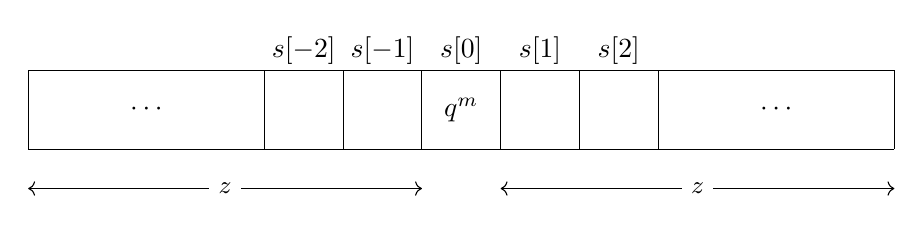
\begin{tikzpicture}
    \draw (0, 1) -- (11, 1);
    \draw (0, 0) -- (11, 0);
    \draw (0, 0) -- (0, 1);
    \draw (11, 0) -- (11, 1);

    \draw (5, 0) -- (5, 1);
    \draw (6, 0) -- (6, 1);
    \draw (4, 0) -- (4, 1);
    \draw (3, 0) -- (3, 1);
    \draw (7, 0) -- (7, 1);
    \draw (8, 0) -- (8, 1);

    \node at (5.5, 1.25) {$s[0]$};
    \node at (6.5, 1.25) {$s[1]$};
    \node at (4.5, 1.25) {$s[-1]$};
    \node at (3.5, 1.25) {$s[-2]$};
    \node at (7.5, 1.25) {$s[2]$};

    \node at (1.5, 0.5) {$\cdots$};
    \node at (9.5, 0.5) {$\cdots$};
    \node at (5.5, 0.5) {$q^m$};

    \path[<->] (6, -0.5) edge node[fill=white, anchor=center, pos= 0.5] {\small $z$} (11, -0.5);
    \path[<->] (0, -0.5) edge node[fill=white, anchor=center, pos =0.5] {\small $z$} (5, -0.5);
  \end{tikzpicture}
\end{center}

\newcommand{\reprt}[1]{\ensuremath{\sim_t^{#1}}}
\newcommand{\reprtt}[2]{\ensuremath{\sim_t^{(#1, #2)}}}
\newcommand{\reprc}{\ensuremath{\sim_c}}

We define the string $E_n$ by the $n$-fold repetition of the blank \blank, followed by the delimiter \#: 
\[ E_n := \underbrace{\blank \ldots \blank}_{n~\text{times}} \#. \]

\begin{definition}[Representation of Half-Tapes]
  Let a part $u$ of a tape be given, i.e.\ $u \in \listsofb{\Sigma}$. The string $h \in \Gamma^{w}$ represents $u$ with polarity $p \in \{-1, 0, 1\}$ and length at most $n$, written $u \reprtt{p}{n} h$, if and only if $\length{u} \le n $ and $h = (\textsf{mapPolarity}~p~u) \concat E_{\hat{n}-\length{u}}$.

  We write $u \reprt{p} h$ for $u \reprtt{p}{z} h$, since $z$ is the length relevant in practice. 
\end{definition}

The more general definition parameterised over the length $n$ is needed for our inductive proofs. 
Note that for $u \reprt{p} h$, we require that $\length{u} \le z$ instead of $\length{u} \le \hat{z}$, which prohibits $M$ from using more space than allowed. 

Obviously $\nil \reprtt{p}{n} E_{\hat{n}}$ for any polarity $p$ (this stems from the fact that blanks are not annotated with polarities).

\begin{definition}[Representation of Configurations]
  Let a configuration $(q, \mathit{tape})$ be given. A string $s$ of length $l$ represents $(q, \mathit{tape})$, written $(q, \mathit{tape}) \reprc s$, if and only if: If
  \begin{itemize}
    \item $\mathit{tape} = \textsf{niltape}$, then $s =  E_z \concat [q^\blank] \concat E_z$, 
    \item $\mathit{tape} = \textsf{leftof}~r~rs$, then there are a polarity $p$ and a string $h$ with $(r :: rs) \reprt{p} h$ such that $s = E_z \concat [q^\blank] \concat h$
    \item $\mathit{tape} = \textsf{rightof}~l~ls$, then there are a polarity $p$ and a string $h$ with $(l::ls) \reprt{p} h$ such that $s = \rev{h} \concat [q^\blank] \concat E_z$, 
    \item $\mathit{tape} = \textsf{midtape}~ls~m~rs$, then there are a polarity $p$ and strings $h_1, h_2$ with $ls \reprt{p} h_1, rs \reprt{p} h_2$ such that $s = \rev{h_1} \concat [q^m] \concat h_2$. 
  \end{itemize}
\end{definition}

These two definitions do exactly capture the intuitive description of the encoding of configurations given above. 

\subsubsection{Correctness of the Simulation}
Now let $R$ be the set of rewriting rules for $M$ given in Section~\ref{sec:rewrules}. We aim to show that the rewriting system given by $R$ and the other parameters fixed before does indeed simulate the Turing machine. We first deal with single simulation steps. For that, we show two directions:
\begin{itemize}
  \item If $(q, \mathit{tape}) \reprc s$ and $(q, \mathit{tape}) \succ (q', \mathit{tape}')$ with $\length{\mathit{tape}} < z'$, then there exists a string $s'$ with $s \strent{} s'$ and $(q', \mathit{tape'}) \reprc s'$. 

    If $(q, \mathit{tape}) \reprc s$ and $q$ is a halting state with $\length{\mathit{tape}} \le z'$, then there exists a string $s'$ with $s \strent{} s'$ and $(q, \mathit{tape}) \reprc s'$. 
  \item If $(q, \mathit{tape}) \reprc s$, $q$ is not a halting state and $s \strent{} s'$, then there exists $(q', \mathit{tape}')$ with $(q', \mathit{tape}') \reprc{} s'$ and $(q, \mathit{tape}) \succ (q', \mathit{tape'})$. 

    If $(q, \mathit{tape}) \reprc s$, $q$ is a halting state and $s \strent{} s'$, then it holds that $(q, \mathit{tape}) \reprc{} s'$. 
\end{itemize}

Note that the second direction is equivalent to the conjunction of the first direction and the rewriting system being deterministic (see Definition~\ref{def:rewdet}) for strings encoding configurations. This will therefore be the way in which we derive the second direction: We prove the first direction and, in addition, uniqueness.

For the uniqueness results, we need inversion results which formulate in which way the given rewrite rules can be applied to a string representing a configuration. 

\begin{lemma}
  There are five regions of a valid configuration string $s$ with $(q, \textsf{tape}) \reprc{} s$ to which different sets of rewrite rules can be applied.
  \begin{itemize}
    \item position $-1$: the rules which apply are exactly those rules which have a state symbol from $\{q^m | q \in Q, m \in \Sigma \cup \{\blank \}\}$ in their center cells
    \item position $0$: the rules which apply are exactly those rules which have a state symbol in their leftmost cells
    \item position $-2$: the rules which apply are exactly those rules which have a state symbol in their rightmost cells
    \item positions $\le -3$: the rules which apply are exactly those rules annotated with  ``both halves'' or ``left half'' above
    \item positions $\ge 1$: the rules which apply are exactly those rules annotated with ``both halves'' or ``right half'' above
  \end{itemize}
\end{lemma}
\begin{proof}
  This is straightforward to prove by case analysis on the used symbols. For the last two cases, we additionally need the invariant given by $\reprt{}$ (and thus $\reprc{}$) that in the left half of a configuration string, there are no blanks right of a non-blank symbol; and in the right half of a configuration string, there are no blanks left of a non-blank symbol.
\end{proof}

\begin{lemma}
  For each state $q \in Q$ of the Turing machine, there exist rules which can be applied at positions $-2, -1$ and $0$. If $q$ is a halting state, the rules for $q$ listed in the ``Halting Extensions'' paragraph can be applied. For the non-halting states, the rules for $q$ listed in the Transitions'' paragraph can be applied.
\end{lemma}

We now first take a look at the parts of a string encoding tape halves.

\begin{definition}[Polarity Reversion]
  \begin{align*}
    \textsf{pRev}~rs := \textsf{rev}~(\textsf{map}~\textsf{pFlip}~rs)
  \end{align*}
  where the function \textsf{pFlip} flips the polarity of elements annotated with a positive or negative polarity and leaves all other elements unchanged.
\end{definition}

\newcommand*{\pRev}[1]{\textsf{pRev}(#1)}

\begin{lemma}\label{lem:taperev}
  Rewrites that are valid for right tape halves are valid for corresponding left tape halves and conversely, rewrites that are valid for left tape halves are valid for corresponding right tape halves.

  In the following, we consider only the rewrite rules for the tape halves (identity, move left, move right). 
  \begin{enumerate}
    \item If $h \strent{} h'$, then also $\pRev{h} \strent{} \pRev{h'}$. 
    \item If $\pRev{h} \strent{} \pRev{h'}$, then also $h \strent{} h'$. 
    \item If $h \strent{} h'$, then also $(\textsf{map}~\textsf{pFlip}~h) \strent{} h'$. 
  \end{enumerate}
\end{lemma}
\begin{proof}
  All of the statements follow via induction due to the definition of the rewrite rules.
\end{proof}

The previous lemma holds because of the symmetry of the rewrite rules for left and right tape halves. It is heavily used throughout the following proofs since it enables us to prove results only for the right tape half, immediately obtaining the symmetric result for the left half as a consequence.

\begin{lemma}[Blank Rewriting]\label{lem:blankrew}
  Let $n \ge w$. Then $E_n \strent{} E_n$. Moreover, $E_{n-1}$ is the unique string with $E_n \strent{} \blank :: E_{n-1}$. 
\end{lemma}

\begin{lemma}\label{lem:blankshiftin}
  Let $n \ge 3$ and $a \in \Sigma$. 
  $E_{n-1}$ is the unique string $s$ satisfying the properties
  \begin{enumerate}
    \item $E_n \strent{} (\polpos{a} :: s)$
    \item $\rev{E_n} \strent{} \rev{(\polneg{a} :: s)}$
  \end{enumerate}
\end{lemma}
\begin{proof}
  The second statement follows immediately from the first one using Lemma~\ref{lem:taperev}.
  For the first statement, since $n \ge 3$, we have to show that $\blank :: \blank :: \blank :: E_{n-3} \strent{} \polpos{a} :: \blank :: \blank :: E_{n-3}$. 
  By Lemma~\ref{lem:blankrew} it holds that $\blank :: \blank :: E_{n-3} \strent{} \blank :: \blank :: E_{n-3}$, and there is no other string $s'$ with $\blank :: \blank :: E_{n-3} \strent{} \blank :: s'$. 
  It therefore remains to show that $\blank\blank\blank \constrent{} \polpos{a}\blank\blank$, and that no other string $s'$ satisfies $\blank :: \blank :: \blank \strent{} \polpos{a} :: s'$. This follows from the rewrite rules given above. 
\end{proof}

\begin{lemma}\label{lem:tapeadd}
  The rewriting system enables us to add one element at the head of one half of the configuration.
  \begin{align*}
    \forall ls~a~h, ls \reprt{} h \rightarrow \length{ls} < z' \rightarrow \exists!~h', \rev{h} \strent{} \rev{(\polneg{a} :: h')} \land a :: ls \reprt{-1} \polneg{a} :: h' \\
    \forall rs~a~h, rs \reprt{} h \rightarrow \length{rs} < z' \rightarrow \exists!~h', h \strent{} \polpos{a} :: h' \land a :: rs \reprt{1} \polpos{a} :: h'
  \end{align*}
\end{lemma}
\begin{proof}
  We prove the second statement, in a generalised form using $\reprtt{p}{n}$ instead of $\reprt{p}$. 
  The first statement can then be derived by applying parts 1 and 3 of Lemma~\ref{lem:taperev}. 
  The proof is by induction on $rs$ with $h$ and $a$ quantified. 

  In the base case, we have $\nil \reprtt{p}{n} h$, therefore $h = E_{\hat{n}}$. We have to show the existence of $h'$ with $h \strent{} \polpos{a} :: h'$ and $[a] \reprtt{1}{n} \polpos{a} :: h'$. $E_{\hat{n}-1}$ does the job, using Lemma~\ref{lem:blankshiftin} for the first conjunct. 

  In the inductive case, we have $r_1 :: rs \reprtt{p}{n} h$ for some polarity $p$ and $\natS{\length{rs}} < n$. We do a case analysis on $rs$. The most interesting case happens when $\length{rs} \ge 2$. Write $rs = \sigma_1 :: \sigma_2 :: rs'$. 
  Since $r_1 :: \sigma_1 :: \sigma_2 ::rs' \reprt{p} h$, it holds that $h = rs_1^p :: \sigma_1^p :: \sigma_2^p :: h''$ by inversion. 
  We have to show the existence of a unique $h_0$ with $r_1^p :: \sigma_1^p :: \sigma_2^p :: h'' \strent{} \polpos{a} :: h_0$ and $a::r_1 :: \sigma_1 :: \sigma_2 :: rs' \reprt{1} \polpos{a} :: h_0$. 

  By the inductive hypothesis for $h := \sigma_1^p :: \sigma_2^p :: h''$ and $a := r_1$, there exists a unique $h'$ with $\sigma_1^p :: \sigma_2^p :: h'' \strent{} \polpos{r_1} :: h'$ and $r_1 :: \sigma_1 :: \sigma_2 :: rs \reprt{1} \polpos{r_1} :: h'$. 
  By an inspection of the rules and inversion, we obtain $h' = \polpos{r_1} :: \polpos{\sigma_1} :: \polpos{\sigma_2} :: H$. 
  Picking $h_0 := \polpos{r_1} :: \polpos{\sigma_1} :: \polpos{\sigma_2} :: H$, we obtain the result with the rule
  \begin{center}
    \rewwin{r_1^p & \sigma_1^p & \sigma_2^p}{\polpos{a} & \polpos{r_1} & \polpos{\sigma_1}}
  \end{center}
  Uniqueness follows by an examination of the rules and the insight that this is the only applicable rule. 
  \end{proof}
\begin{lemma}\label{lem:taperem}
  The rewriting system enables us to remove one element at the head of one half of the configuration.
  \begin{align*}
    \forall ls~a~b~h, a::b::ls \reprt{} a::b::h \rightarrow \exists!~h', \rev{(a :: b :: h)} \strent{} \rev{(\polpos{b} :: h')} \land b :: ls \reprt{1} \polpos{b} :: h' \\
    \forall rs~a~b~h, a :: b :: rs \reprt{} a :: b :: h \rightarrow \exists!~h', a :: b :: h \strent{} \polneg{b} :: h' \land b :: rs \reprt{-1} \polneg{b} :: h'
  \end{align*}
\end{lemma}
\begin{proof}
  Uses the same style of arguments as Lemma~\ref{lem:tapeadd}.
\end{proof}

\begin{lemma}\label{lem:tapeid}
  The rewriting system enables us to leave tape halves unchanged. 
  \begin{align*}
    \forall ls~a~h, a :: ls \reprt{} a :: h \rightarrow \exists !~h', \rev{(a::h)} \strent{} \rev{(\polneut{a} :: h')} \land a :: ls \reprt{0} \polneut{a} :: h'\\
    \forall rs~a~h, a :: rs \reprt{} a :: h \rightarrow \exists !~h', a :: h \strent{} \polneut{a} :: h' \land a :: rs \reprt{0} \polneut{a} :: h'
  \end{align*}
\end{lemma}
\begin{proof}
  Uses the same style of arguments as Lemma~\ref{lem:tapeadd}.
\end{proof}

The key insight behind the proofs for these results is that the successor tape string is uniquely determined by the polarity of the symbol at the head of the successor string. 

\begin{lemma}\label{lem:simstep}
  Let $(q, \mathit{tape}) \reprc{} s$ and $(q, \mathit{tape}) \succ (q', \mathit{tape}')$ with $\length{\mathit{tape}} < z$. There exists a uniquely determined string $s'$ with $s \strent{} s'$. $s'$ satsifies $(q', \mathit{tape}') \reprc{} s'$. 
\end{lemma}
\begin{proof}
  By case analysis on the transition the Turing machine takes. This transition is uniquely determined. We then mimic this transition in the rewriting system using a suitable rewrite window with the state at the center cell. If the tape is moved, we'll have to look ahead at two neighbouring symbols in the opposite direction of the move; therefore we need further case analyses. We can then apply the previous two lemmas in order to obtain unique successors for the tapes. 
  We then finish the proof by using the rewrite windows having a state symbol in the outer cells. 

  Let's take a look at a few of the cases.
  We first do a case analysis on $\mathit{tape}$.
  \begin{description}
    \item[$\textsf{midtape}~ls~m~rs$:]
      It is known by $(q, \mathit{tape}) \reprc{} s$ that $s = \rev{h_1} \concat [q^m] \concat h_2$ for $ls \reprt{p} h_1$ and $rs \reprt{p} h_2$.

      Case analysis on the transition.
      \begin{description}
        \item[$\delta(q, m) = (q', m', \textsf{L})$:]
          The head should move left on the tape, therefore the tape must be shifted to the right. We aim to apply a rule of the form
          \begin{center}
            \rewwin{x_1^p & q^m & x_3^p}{\polpos{x_2} & {q'}^{x_1} & \polpos{m'}}
          \end{center}
          where the $x_i$ denote symbols which are either blanks or elements of $\Sigma$ and we now have explicitly annotated the polarities. We have to do a case analysis on these symbols in order to find out which rule we need to apply. 
          The rule we need to apply is then uniquely determined. 

          Here, the case where $ls = \sigma_1 :: \sigma_2 :: lsr$ and $rs = \sigma_3 :: rsr$ is considered, implying that $h_1 = \sigma_1^p :: \sigma_2^p :: LS$ and $h_2 = \sigma_3^p :: RS$. 
          This means that $x_1 = \sigma_1, x_2 = \sigma_2$ and $x_3 = \sigma_3$. The rule 
          \begin{center}
            \rewwin{\sigma_1^p & q^m & \sigma_3^p}{\polpos{\sigma_2} & {q'}^{\sigma_1} & \polpos{m'}}
          \end{center}
          can now be used.

          Next, we transform the two halves of the tape according to the Lemmas~\ref{lem:tapeadd} and~\ref{lem:taperem}. The element $m'$ needs to be added to the right half, while the element $\sigma_1$ has to be removed from the left one. 
          For the right half, we get a unique $RS'$ such that 
          \[\sigma_3^p :: RS \strent{} \polpos{m'} :: \polpos{\sigma_3} :: RS' \text{ and } m' :: \sigma_3 :: rsr \reprt{1} \polpos{m'} :: \polpos{\sigma_3} :: RS'.\]
          Similarly, for the left half, there is a unique $LS'$ such that 
          \[\rev{\sigma_1^p :: \sigma_2^p :: LS} \strent{} \rev{\polneg{\sigma_2} :: LS'} \text{ and } \sigma_2 :: lsr \reprt{1} \polpos{\sigma_2} :: LS'.\]

          We now want to show that 
          \[\rev{(\sigma_1^p :: \sigma_2^p :: LS)} \concat [q^m] \concat (\sigma_3^p :: RS) \strent{} \rev{(\polpos{\sigma_2} :: LS')} \concat [{q'}^{\sigma_1}] \concat (\polpos{m'} :: \polpos{\sigma_3} :: RS') \]
          and 
          \[ 
            (q', \mathit{tape}') \reprc{} \rev{(\polpos{\sigma_2} :: LS')} \concat [{q'}^{\sigma_1}] \concat (\polpos{m'} :: \polpos{\sigma_3} :: RS') 
          \]
          where $\mathit{tape}'$ is the new tape obtained by $\textsf{doAct}~\mathit{tape}~(\Some{m'}, \textsf{L})$, i.e.\ 
          \[\mathit{tape}' = \textsf{midtape}~(\sigma_2 :: lsr)~\sigma_1~(m' :: \sigma_3 :: rsr).\]

          The latter is straightforward to prove. For the former, we have to show that at every offset of the the configuration strings, we can apply a valid rewrite window. We have already shown that for the position $-1$ as well as (by the transformations of the tape halves) for positions $\le -3$ and $\ge 1$ (where we consider these positions wrt.\ the left border of the window).
          For position $-2$ we have to use a window which has a state symbol in its rightmost cells, for position $0$ we have to use a window which has a state symbol in its leftmost cells.

          For both proofs, we have to do a case analysis on $lsr$ or $rsr$, respectively; apart from that, the proof is straightforward with the rules constructed for the given transition.
      \end{description}
    \item[$\textsf{leftof}~r~rs$:]
    	Arguments are similar in style to the previous case. 
    \item[$\textsf{rightof}~l~ls$:]
    	Arguments are similar in style to the previous case. 
    \item[$\textsf{niltape}$:]
      It is known by $(q, \mathit{tape}) \reprc s$ that $s = \rev{E_{\hat{z}}} \concat [q^\blank] \concat E_{\hat{z}}$. 
      Of course, $[] \reprc{} E_{\hat{z}}$.
      Case analysis on the transition. 
      \begin{description}
        \item[$\delta(q, \None) = (q', \Some{a}, \textsf{R})$:]
          The head should move right on the tape, therefore the tape must be shifted to the left. We aim to apply the rule 
          \begin{center}
            \rewwin{\blank & q^\blank & \blank}{\polneg{a} & {q'}^\blank & \blank}
          \end{center}
          We only need to transform the left half of the tape. 
          By Lemma~\ref{lem:tapeadd}, there exists a unique string $ls'$ with $\rev{E_{\hat{z}}} \strent{} \rev{\polneg{a}:: ls'}$ and $[a] \reprt{-1} \polneg{a} :: ls'$. In fact, $ls' = E_{\hat{z}-1}$. 
          Moreover, by Lemma~\ref{lem:blankrew}, $E_{\hat{z}} \strent{} E_{\hat{z}}$ and $[] \reprt{-1} E_{\hat{z}}$.
          Thus, it again remains to consider the positions $-2$ and $0$. Both follow by a straightforward examination of the rules.
      \end{description}
  \end{description}
\end{proof}

As can be seen from this outline, the proof mostly consists of an armada of case analyses\sarcasm{Really, no one would have expected that after reading all the different rules for rewrite windows, right?}.

We now still have to consider the case where $q$ is a halting state. 
\begin{lemma}\label{lem:haltextstep}
  Let $(q, \mathit{tape}) \reprc{} s$ where $q$ is a halting state, then there exists a uniquely determined string $s'$ with $s \strent{} s'$. $s'$ satisfies $(q, \mathit{tape}) \reprc{} s'$. 
\end{lemma}
\begin{proof}
  Completely analogous to the cases of Lemma~\ref{lem:simstep} where the tape is not moved.
\end{proof}

The other direction now follows from the uniqueness properties. 

\begin{lemma}[Step Inversion]\label{lem:stepinv}
  If $(q, \mathit{tape}) \reprc{} s$, $q$ is not a halting state and $s \strent{} s'$, then there exists a uniquely determined successor configuration $(q', \mathit{tape}')$ with $(q', \mathit{tape}') \reprc{} s'$ and $(q, \mathit{tape}) \succ (q', \mathit{tape}')$. 
\end{lemma}
\begin{proof}
  Since the Turing machine is deterministic and $q$ is not halting, the existence of unique $(q', \mathit{tape}')$ with $(q, \mathit{tape}) \succ (q', \mathit{tape}')$ follows directly. By Lemma~\ref{lem:simstep}, there is a uniquely determined string $s''$ with $s \strent{} s''$ and $(q', \mathit{tape}') \reprc{} s''$. Since $s \strent{} s'$, too, it follows that $s' = s''$ by uniqueness.
\end{proof}

\begin{lemma}[Halting Inversion]\label{lem:haltinv}
  If $(q, \mathit{tape}) \reprc{} s$, $q$ is a halting state and $s \strent{} s'$, then $(q, \mathit{tape}) \reprc{} s'$. 
\end{lemma}
\begin{proof}
  Follows directly from Lemma~\ref{lem:haltextstep}. 
\end{proof}

The above results can be easily extended to multiple simulation steps. 
\begin{lemma}[Multi-step Simulation]\label{lem:mssim}
  Let $(q, \mathit{tape}) \reprc{} s$ and $(q, \mathit{tape}) \succ^k (q', \mathit{tape}')$ for some $k \ge 0$ and $\mathit{tape} \le z - k$. There exists a uniquely determined string $s'$ with $s \strent^k s'$ and $(q', \mathit{tape}') \reprc{} s'$. 
\end{lemma}
\begin{proof}
  By induction on $k$, using Lemma~\ref{lem:simstep} in the inductive step.
\end{proof}

\begin{lemma}[Halting Extension]\label{lem:haltext}
  Let $(q, \mathit{tape}) \reprc{} s$ for a halting state $q$ and $k \ge 0$. There exists a unique $s'$ with $s \strent{}^k s'$ and $(q, \mathit{tape}) \reprc{} s'$. 
\end{lemma}
\begin{proof}
  By induction on $k$. The case for $k = 0$ is trivial.
  Otherwise, we have the existence of a unique $s'$ with $s \strent^k s'$ and $(q, \mathit{tape}) \reprc{} s'$ by the inductive hypothesis. An application of Lemma~\ref{lem:haltextstep} yields the result.
\end{proof}

\begin{lemma}[Multi-step Inversion]\label{lem:multiinv}
  Let $(q, \mathit{tape})$ and $s$ with $(q, \mathit{tape}) \reprc{} s$ be given. If $s \strent^{j} s'$, then there exists $(q', \mathit{tape}')$ with $(q', \mathit{tape}') \reprc{} s'$ and a $j' \le j$ with $(q, \mathit{tape}) \succ^{j'} (q', \mathit{tape}')$, $\length{\mathit{tape}'} \le \length{\mathit{tape}} + j'$. 
\end{lemma}
\begin{proof}
  The proof is by induction on $j$, with $s'$ quantified. 
  If $j = 0$, then $s = s'$ and the claim is trivial for $j' = 0$.

  Otherwise, we have $s \strent^{j+1}$, thus $s \strent^{j} s''$ and $s'' \strent{} s'$. By the inductive hypothesis, there exists $(q'', \mathit{tape}'')$ with $(q'', \mathit{tape}'') \reprc{} s''$, $(q, \mathit{tape}) \succ^{j''} (q'', \mathit{tape}'')$ and $\length{\mathit{tape''}} \le \length{\mathit{tape}} + j''$. 

  If $q''$ is a halting state, then by Lemma~\ref{lem:haltinv} $(q'', \mathit{tape}'') \reprc{} s'$. We thus choose $(q', \mathit{tape}') = (q'', \mathit{tape}'')$ and $j' = j''$. 

  Otherwise, by Lemma~\ref{lem:stepinv}, there exists a uniquely determined $(q', \mathit{tape}')$ with $(q', \mathit{tape}') \reprc{} s'$ and $(q'', \mathit{tape}'') \succ (q', \mathit{tape}')$. 
  Choosing $j' := \natS{j''}$ finishes the proof.
\end{proof}


\begin{lemma}[Final Condition]\label{lem:finalcond}
  Let $(q, \mathit{tape}) \reprc{} s$. Then $q$ is halting if, and only if, $s \models \Rfinal$. 
\end{lemma}

Now, it can be shown that the simulation is sound and complete.

\begin{theorem}[Completeness]\label{thm:simcomplete}
  Let a configuration $(q, \mathit{tape})$ be given with $\length{\mathit{tape}} \le k$. Then there exists a string $s$ with $(q, \mathit{tape}) \reprc{} s$. If $(q, \mathit{tape}) \rhd^{\le t} (q', \mathit{tape}')$, then there exists a string $s'$ with $s \strent{}^t s'$ and $(q', \mathit{tape}') \reprc{} s'$.  
\end{theorem}
\begin{proof}
  The existence of the string $s$ follows by the definition of $\reprc{}$ (the relation directly induces a functional definition).  
  For the second statement, let $(q, \mathit{tape}) \rhd^{t'} (q', \mathit{tape}')$ for $t' \le t$. 
  This implies that $(q, \mathit{tape}) \succ^{t'} (q', \mathit{tape}')$ and that $q'$ is a halting state. 
  By Lemma~\ref{lem:mssim}, there exists a uniquely determined string $s'$ with $s \strent^{t'} s'$ and $(q', \mathit{tape}') \reprc{} s'$. An application of Lemma~\ref{lem:haltext} yields the existence of a unique $s''$ with $s' \strent^{t - t'} s''$ and $(q', \mathit{tape}') \reprc{} s''$.
\end{proof}

  

\begin{theorem}[Soundness]\label{thm:simsound}
  Let a string $s$ be given such that there exists a configuration $(q, \mathit{tape})$ with $(q, \mathit{tape}) \reprc{} s$ and $\length{\mathit{tape}} \le k$. If $s \strent^t s'$ and $s' \models \Rfinal$, then there exists a configuration $(q', \mathit{tape}')$ with $(q', \mathit{tape}') \reprc{} s'$ such that $(q, \mathit{tape}) \rhd^{\le t} (q', \mathit{tape}')$ and $\length{\mathit{tape}'} \le z$. 
\end{theorem}
\begin{proof}
  By Lemma~\ref{lem:multiinv} and Lemma~\ref{lem:finalcond} for the final condition.
\end{proof}

%\TODO{Is it really a good idea to explicitly spell out this intermediate step?}
We can now give a reduction from \gennp{} to a first variant of \strconrew{}, where we still haven't resolved the nondeterminism of choosing an initial tape state:
\begin{definition}[\textbf{GenNP-IntermediateTape}]\label{def:gennpinter}
  Given: alphabets $\Gamma$ and $\Sigma \subseteq \Gamma$, a time bound $t$, a set of rewrite windows $R$, final constraints $\Rfinal$, and a Turing machine state $q$ and a number $k$. 
  Determine if there exists a string $\mathit{input}$ over $\Sigma$ of length $\length{\mathit{input}} \le k$ such that 
  \[(\Gamma, 2 (t + k + 3) + 1, t, \textsf{initConf}~q~(\textsf{initTape}~\mathit{input}), 3, 1, R, \Rfinal) \in \strconrew{},\]
  where $\textsf{initConf}$ just computes a canonical string $s$ with $(q, \textsf{initTape}~\mathit{input}) \reprc{} s$. 
\end{definition}
\begin{theorem}[Reduction to Intermediate Parallel Rewriting Problem]
  There is a polynomial-time reduction from \gennp{} to \textbf{GenNP-IntermediateTape}. 
\end{theorem}
\begin{proof}
  The construction and correctness follow the description in this subsection. 
  It's intuitively clear that the rewrite rules can be computed in polynomial time since their structure directly follows the structure of the Turing machine transition function. 

  For the correctness, we prove the two directions. 
  \begin{description}
    \item[$\Rightarrow$:]
      Let $(M, k, t) \in \gennp{}$. Therefore, there is an input $x$ of length $\length{x} \le k$ such that there is a halting configuration $c$ with $(\mathit{start}, \textsf{initTape}~x) \rhd^{\le t} c$. Define $s := \textsf{initConf}~\mathit{start}~(\textsf{initTape}~x)$.  

      It holds that $(\mathit{start}, \textsf{initTape}~x) \reprc{} s$. 
      Moreover, $c = (q', \mathit{tape}')$ with $\length{\mathit{tape}'} \le z$, since $\mathit{tape}' \le t + k$ by ``time bounds space'' for Turing machines. By Theorem~\ref{thm:simcomplete}, there exists a string $s'$ with $s \strent{} s'$ and $(q', \mathit{tape}') \reprc{} s'$. Since $q'$ is a halting state by assumption and the symbol ${q'}^m$ is contained in $s'$ by definition of $\reprc{}$ for some $m \in \Sigma \cup \{\blank\}$, it holds by construction that $s' \models \Rfinal$, making the \textbf{GenNP-IntermediateTape} instance accepting.

    \item[$\Leftarrow$:]
      Let there be $\mathit{input}$ over $\Sigma$ with $\length{\mathit{input}} \le k$, such that the given instance of \strconrew{} is contained in \strconrew{}. This means that there is $s'$ with $s \strent{}^t s'$ for $s := \textsf{initConf}~q~(\textsf{initTape}~\mathit{input})$ and $s' \models \Rfinal$.  
      By construction, $(q, \textsf{initTape}~\mathit{input}) \reprc{} s$. Theorem~\ref{thm:simsound} asserts the existence of $(q', \mathit{tape}')$ with $(q', \mathit{tape}') \reprc{} s'$ with $(q, \textsf{initTape}~\mathit{input}) \rhd^{\le t} (q', \mathit{tape}')$. Since $s' \models \Rfinal$, by construction, we have that $q'$ is an accepting state of the Turing machine. This implies that the original \gennp{} instance is a positive instance, too.
  \end{description}
\end{proof}


\subsection{Interlude: A Recipe for Adding Preludes to \strconrew{}}
In this section, we introduce a technique for generating an initial string $x_0$ for \strconrew{} instances (we will call this process the \emph{prelude} of the resulting \strconrew{} instance) by expanding the alphabet and adding new rules to the system. The rules have to be designed such that, from a new initial string $x_0'$, exactly $t'$ rewrite steps can be done using the new rules (and the original rules cannot be applied to any intermediate string encountered during these steps), before ending up with a ``new'' initial string for the original \strconrew{} instance (and from there on, the new rules cannot be applied anymore). 
This technique will, for instance, allow us to handle the nondeterministic input string of our Turing machines, by being able to reduce the question
\begin{center}
  ``Does there exist an initial input string $x_0$ of a certain form such that a rewrite with $t$ steps to a final string satisfying $\Rfinal$ is possible?''
\end{center}
to the simpler question
\begin{center}
  ``For a fixed input $x_0'$, can $x_0'$ be rewritten in $t + t'$ steps to a final string satisfying $\Rfinal$?''
\end{center}
This will be enabled by using nondeterministic rewrite rules that can generate an input to the Turing machine simulation.

Let us fix a partial rewriting system $S = (\Sigma, l, t, w, o, R, \Rfinal)$ (i.e.\ a rewriting system missing an initial string) throughout this subsection. 
First of all, we define compatibility and disjointness of rules. 
\begin{definition}[Compatibility]
  Let an alphabet $\Sigma'$, a set of rules $R'$ and an initial string $s_0 \in \listsofb{\Sigma'}$ be given. 
  The triple $(\Sigma', R', s_0)$ is compatible with $S$ if
  \begin{itemize}
    \item the rules in $R'$ have width $w$
    \item $\length{s_0} = l$
  \end{itemize}
\end{definition}
\begin{definition}[Disjointness]
  Let an alphabet $\Sigma'$, a set of rules $R'$ and an initial string $s_0 \in \listsofb{\Sigma'}$ be given. 
  The triple $(\Sigma', R, s_0)$ is disjoint from $S$ if 
  \begin{itemize}
    \item $\Sigma \cap \Sigma' = \emptyset$
    \item the rules $a \constrent{} b \in  R'$ all have premises which are strings over $\Sigma'$, i.e.\ $a \in \listsofb{\Sigma'}$
    \item $s_0 \in \listsofb{\Sigma'}$
  \end{itemize}
\end{definition}

Intuitively, compatibility ensures that the prelude fits the existing rewrite system $S$ and disjointness enables nice correctness results by ensuring that rules of the prelude cannot be applied after the prelude, and that existing rules from $R$ cannot be used when only rules of the prelude are allowed. 

\begin{definition}[Prelude]
  Let $\Sigma', R', s_0$ be given such that $(\Sigma', R', s_0)$ satisfies compatibility and disjointness for $S$. 
  For a number of \emph{prelude steps} $t'$, $P = (\Sigma', R', t', s_0)$ is a prelude for $S$ if the following condition is satisfied:
  \[\forall s_1, \ldots, s_{t'}, (\forall 0 \le i < t', s_i \strent_{R'} s_{i+1}) \rightarrow (\forall 0 < i < t', s_i \in \listsofb{\Sigma'}) \land s_{t'} \in \listsofb{\Sigma} \]
  (where the relation $\strent_{R'}$ is wrt.\ to the new rules $R'$) %TODO: not that it makes a difference
\end{definition}
The condition for a prelude ensures that the ``timing'' of the new rules is exactly predictable, by ensuring that after exactly $t'$ steps with the new rules, existing rules can be applied. We say that the prelude closes after $t'$ steps. 

\begin{definition}[Soundness and Completeness]
  A prelude $P$ for $S$ is complete with respect to an initial condition $p : \listsofb{\Sigma} \rightarrow \Prop$, if
  \[ \forall x_0, p~x_0 \rightarrow (\Sigma', l, t', s_0, w, o, R', \{x_0\}) \in \strconrew{}. \]
  $P$ is sound for $p$, if 
  \[ \forall x_0, (\Sigma', l, t', s_0, w, o, R', \{x_0\}) \in \strconrew{} \rightarrow p~x_0. \]
\end{definition}

Soundness and completeness say that $P$ can generate exactly those strings in $t'$ steps for which $p$ holds. 

Using these definitions, we obtain the following central result:
\begin{lemma}\label{lem:prelude}
  Let a predicate $p$ and a prelude $P$ be given such that $P$ is sound and complete for $p$. 
  Define $S' := (\Sigma \sqcup \Sigma', l, t + t', s_0, w, o, R \cup R', \Rfinal)$.
  Then 
  \[(\exists x_0, p~x_0 \land (\Sigma, l, t, x_0, w, o, R, \Rfinal) \in \strconrew{}) \leftrightarrow S' \in \strconrew{}. \]
\end{lemma}

%\subsection{Normalising Tapes}
%In this subsection we show that we can restrict ourselves wlog to initial tape states for which the tape head initially resides to the left of the input. 
%\TODO{proceeds using nondeterministic rewrite rules that allow $k$ shifts of the tape; main challenge is that this needs to always take a fixed number of rewrite steps. for that, use a counter that is decreased with each shift. if the counter reaches zero, a final rewrite brings the string into a state on which the TM simulation can run}

%\begin{definition}[\textbf{GenNP-IntermediateNormTape}]
  %Given: alphabets $\Gamma$ and $\Sigma \subseteq \Gamma$, a time bound $t$, a set of rewrite windows $R$, final constraints $\Rfinal$, and a Turing machine state $q$ and a number $k$. 
  %Determine if there exists an input string $\mathit{input}$ over $\Sigma$ with $\length{\mathit{input}} \le k$ such that 
  %\[(\Gamma, 2 (t + k + 3) + 1, t, \textsf{initConf'}~q~\mathit{input}, 3, 1, R, \Rfinal) \in \strconrew{}.\]
  %\TODO{the important property here is that initConf' will generate either a leftof tape or a niltape}
%\end{definition}

%\TODO{the proof is implemented as a prelude as described in the previous section}

\subsection{Introducing Nondeterminism}\label{sec:nondet}
In this section we finally reduce \textbf{GenNP-IntermediateNormTape} to \strconrew{}\sarcasm{Yay!}. 

The basic idea is to take create an initial string containing special symbols $\top$ where input symbols for the Turing machine can be placed. Then, we add nondeterministic rewrite rules that allow these symbols to be guessed in a single rewrite step. Thus, after a single step, we end up with a valid initial configuration string for the Turing machine simulation.

The new initial string $x_0'$ looks as follows, for symbols $\top, \bot, \underline{q^\blank}, \underline{\#}$ not contained in the alphabet $\Gamma$, where $q$ is the desired initial state:
\begin{center}
  \begin{tikzpicture}
    \draw (0, 0.5) -- (10.5, 0.5);
    \draw (0, 0) -- (10.5, 0);
    \draw (0, 0) -- (0, 0.5);
    \draw (10.5, 0) -- (10.5, 0.5);

    \draw (0.5, 0.5) -- (0.5, 0);
    \draw (1, 0.5) -- (1, 0);
    \draw (10, 0.5) -- (10, 0);
    \draw (9.5, 0.5) -- (9.5, 0);
    \draw (5, 0.5) -- (5, 0);
    \draw (5.5, 0.5) -- (5.5, 0);
    \draw (4.5, 0.5) -- (4.5, 0);
    \draw (6, 0.5) -- (6, 0);
    \draw (7.5, 0.5) -- (7.5, 0);
    \draw (8, 0.5) -- (8, 0);
    \draw (8.5, 0.5) -- (8.5, 0);
   
    \node at (0.25, 0.25) {\#};
    \node at (0.75, 0.24) {$\bot$};
    \node at (4.75, 0.25) {$\bot$};
    \node at (5.25, 0.25) {$\underline{q^\blank}$};
    \node at (5.75, 0.25) {$\top$};
    \node at (7.75, 0.25) {$\top$};
    \node at (8.25, 0.25) {$\bot$};
    \node at (9.75, 0.25) {$\bot$};
    \node at (10.25, 0.25) {\#};

    \path[<->] (5.5, -0.5) edge node[fill=white, anchor=center, pos= 0.5] {\small $k$} (8, -0.5);
    \path[<->] (0, -0.5) edge node [fill = white, anchor=center, pos=0.5] {\small $t + k + 3$} (5, -0.5);
    \path[<->] (8, -0.5) edge node [fill = white, anchor =center, pos=0.5] {\small $t + 3$} (10.5, -0.5);
  \end{tikzpicture}
\end{center}

The symbol $\top$ denotes positions where elements of the tape alphabet $\Sigma$ may be placed, $\bot$ denotes positions where blanks must be placed. While the string could, in principle, also directly contain blanks \blank{}, a string with no symbols of the old alphabet $\Gamma$ will make proofs more convenient. 

Designing the rewriting rules is now straightforward. The only part which takes some consideration is the fact that the input string may be shorter than $k$ symbols, but there may never be blanks inbetween elements of the tape alphabet. This difficulty is easily resolved due to the overlapping rewrite windows:
\begin{center}
  \rewwin{\bot & \bot & \bot}{\blank & \blank & \blank}
  \rewwin{\underline{\#} & \bot & \bot}{\# & \blank & \blank}
  \rewwin{\bot & \bot & \underline{\#}}{\blank & \blank & \#} \\[3ex]
  \rewwin{\bot & \bot & \underline{q^\blank}} {\blank & \blank & q^\blank}
  \rewwin{\bot & \underline{q^\blank} & \top}{\blank & q^\blank & \polneut{m_1}}
  \rewwin{\bot & \underline{q^\blank} & \bot}{\blank & q^\blank & \blank} \\[3ex]
  \rewwin{\underline{q^\blank} & \bot & \bot}{q^\blank & \blank & \blank} 
  \rewwin{\underline{q^\blank} & \top & \bot}{q^\blank & \polneut{m_1} & \blank}
  \rewwin{\underline{q^\blank} & \top & \top}{q^\blank & \polneut{\sigma_1} & \polneut{m_1}}
  \rewwin{\underline{q^\blank} & \top & \top}{q^\blank & \blank & \blank} \\[3ex]
  \rewwin{\top & \top & \top}{\polneut{\sigma_1} & \polneut{\sigma_2} & \polneut{m_1}}
  \rewwin{\top & \top & \top}{\polneut{\sigma_1} & \blank & \blank} 
  \rewwin{\top & \top & \top}{\blank & \blank & \blank} \\[3ex]
  \rewwin{\top & \top & \bot}{\polneut{\sigma_1} & \polneut{m_1} & \blank}
  \rewwin{\top & \top & \bot}{\blank & \blank & \blank} 
  \rewwin{\top & \bot & \bot}{\polneut{m_1} & \blank & \blank}
  \rewwin{\top & \bot & \bot}{\blank & \blank & \blank} \\[3ex]
\end{center}

These rules enforce that if we decide to replace a $\top$ with a blank instead of an element from $\Sigma$, all $\top$'s to the right of it will also need to be replaced by blanks. After one step, a configuration with state $q$ and a tape which either represents a \textsf{niltape} or a \textsf{leftof} tape of length $\le k$ is generated. 
We will refer to the set of these rules as $R'$.

Our goal now is to show that these new rules consitute a sound and complete prelude for incomplete rewriting system 
\[S = (\Gamma, 2(t + k + 3) + 1, t, , 3, 1, R, \Rfinal)\]
of Definition~\ref{def:gennpinter}, missing an input which has to be of the form 
\[ \textsf{initConf}~q~(\textsf{initTape}~\mathit{input}) \]
for an input string $\mathit{input}$ with $\length{\mathit{input}} \le k$ for the Turing machine simulation.

\begin{lemma}
  The above construction is a prelude for $S$ in one step. 
\end{lemma}
\begin{proof}
  Disjointness and compatiblity are obvious. 
  Now let $s_1$ be given with $s_0 \strent_{R'} s_1$. We need to show that $s_1 \in \Gamma^l$ for $l = 2 (t + k + 3) + 1$. 
  This easily follows from the fact that the conclusions of the rewrite rules only contain elements of $\Gamma$.
\end{proof}

\begin{lemma}\label{lem:nondetsc}
  $(\{\top, \bot, \underline{q^\blank}, \underline{\#}\}, R', 1, x_0')$ is sound and complete for $p$, where $p : \listsofb{\Gamma} \rightarrow \Prop$ is defined as follows: 
  \[p~s := \exists \mathit{input}, \length{\mathit{input}} \le k \land s = \textsf{initConf}~q~(\textsf{initTape}~\mathit{input})\]
\end{lemma}
\begin{proof}
  We have to show two directions:
  \begin{description}
  	\item[Completeness:]
      Let $x_0$ be an initial string such that there is a string $s$ with $\length{s} \le k$ and $x_0 = \textsf{initConf}~q~(\textsf{initTape}~s) = E_{\hat{z}} \concat [q^\blank] \concat s \concat E_{\hat{z} - \length{s}}$, where we implicitly lift the string $s$ from $\Sigma$ to $\Sigma'$. We have to show that the new initial string $x_0'$ can be rewritten to $x_0$, that is, $x_0' \strent{} x_0$, using the new rules $R'$. As for the simulation of deterministic Turing machines, we split the proof by showing that the rewrites for the two tape halves are valid.

      For the left half, this is trivial, as all $\bot$'s can be replaced by \blank's (a simple inductive proof over $z$ suffices). The hard part is the right tape half where the initial input string has to be placed.
      We first show that 
      \[ \forall w, \underbrace{\top \ldots \top}_{\length{s}} \underbrace{\top \ldots \top}_{w} \underbrace{\bot \ldots \bot}_{t + 2}\underline{\#} \strent{} s \concat \underbrace{\blank \ldots \blank}_{w} \underbrace{\blank \ldots \blank}_{t+2}\# \]
      by induction on $s$. The desired result that 
      \[\underbrace{\top \ldots \top}_{k} \underbrace{\bot \ldots \bot}_{t+2}\underline{\#} \strent{} s \underbrace{\blank \ldots \blank}_{k-\length{s}} \underbrace{\blank \ldots \blank}_{t+2}\# \]
      then follows by setting $w := k - \length{s}$. 

      Finally, arguing about the center position proceeds as usual via case analyses.

  	\item[Soundness:]
      Let $x_0' \strent{} x_0$ using the rules in $R'$. We need to show that $p~x_0$ holds, i.e.\ there exists $s$ with $x_0 = \textsf{initConf}~q~(\textsf{initTape}~s)$ and $\length{s} \le k$. 
      
      The statement for the left tape half follows trivially from the available rewrite rules, by an induction on the length of the string. 

      For the right tape half we have to show
      \[\underbrace{\top \ldots \top}_{k} \underbrace{\bot \ldots \bot}_{t + 2}\underline{\#} \strent{} w \rightarrow \exists s, \length{s} \le k \land w = s_1 \ldots s_{\length{s}} \underbrace{\blank \ldots \blank}_{k-\length{s}} \underbrace{\blank \ldots \blank}_{t + 2}\#. \]
      If $k \ge 3$, it suffices to show that ${\bot}^{t+2}\underline{\#} \strent{} w \rightarrow w = \blank \ldots \blank\#$ and ${\top}^k \strent{} w \rightarrow \exists s, w = s \concat \blank \ldots \blank$. Both statements follow by induction on the length of the first string. The overlapping windows then don't matter to us since the other windows already uniquely determine the string. 

      In the case of $k < 3$, the statement for the $\top$ part falls apart since strings of length $< 3$ can be vacuously rewritten to any arbitrary string (since there is no rewrite rule with a matching premise). We then have to consider the overlapping rules to derive the statement.
  \end{description}
\end{proof}

\begin{theorem}
  There is a polynomial-time reduction from \textbf{GenNP-IntermediateTape} to \gennp{}. 
\end{theorem}
\begin{proof}
  Follows with Lemma~\ref{lem:nondetsc} and Lemma~\ref{lem:prelude}.
\end{proof}

\section{Reducing \strconrew{} to \binstrconrew{}}
\TODO{outline the needed homomorphism and justification}

Conjecture: Parallel Rewriting is invariant under injective homomorphisms which map all symbols to strings of the same length

\section{Encoding Rewriting Systems as Circuits: Reduction to \csat{}}
\TODO{give the main construction ideas}

\section{Reducing \csat{} to \sat{}}
\TODO{Outline of Tseytin transformation; can adapt and expand the DNF procedure from ICL2019}

\section{Related Work}
\TODO{mainly Heiter's Bachelor thesis; comment on TM -> SR reduction and why their SR problem isn't suitable for our setting}

\section{Formalisation}
List of notes and TODOs:
\begin{itemize}
  \item might unfold the lists in definition of valid
  \item maybe separate rules for 0, 1, 2 in valid
  \item maybe length as parameter in valid
\end{itemize}

\appendix
\section{Missing Rewrite Rules}
\paragraph*{$\delta(q, \Some{a}) = (p, \None, \textsf{R})$:}
\begin{center}
  \rewwin{m_1 & q^a & \blank}{\polneg{a} & p^{\blank} & \blank}
  \rewwin{m_1 & q^a & \sigma_1}{\polneg{a} & p^{\sigma_1} & \polneg{m_2}} \\[3ex]
  \rewwin{q^a & \blank & \blank}{p^{\blank} & \blank & \blank}
  \rewwin{q^a & \sigma_1 & \blank}{p^{\sigma_1} & \blank & \blank}
  \rewwin{q^a & \sigma_1 & \sigma_2}{p^{\sigma_1} & \polneg{\sigma_2} & \polneg{m_1}} \\[3ex]
  \rewwin{\blank & \blank & q^a}{\blank & \polneg{a} & p^{m_1}}
  \rewwin{m_1 & \sigma_1 & q^a}{\polneg{\sigma_1} & \polneg{a} & p^{m_2}}
\end{center}

\paragraph*{$\delta(q, \Some{a}) = (p, \None, \textsf{N})$:}
\begin{center}
  \rewwin{m_1 & q^a & m_2}{\polneut{m_1} & p^a & \polneut{m_2}} \\[3ex]
  \rewwin{q^a & \sigma_1 & m_1}{p^a & \polneut{\sigma_1} & \polneut{m_1}}
  \rewwin{q^a & \blank & \blank}{p^a & \blank & \blank} \\[3ex]
  \rewwin{m_1 & \sigma_1  & q^a}{\polneut{m_1} & \polneut{\sigma_1} & p^a} 
  \rewwin{\blank & \blank & q^a}{\blank & \blank & p^a}
\end{center}

\section{Semantics of Turing Machines}
\TODO{more on semantics of Turing machines}

\bibliography{memo}{}


\end{document}
